\chapter{Tests}\label{ch:tests}
\section{Introduction}\label{sec:tests:introduction}
Don Norman, in his book \say{The Design of Everyday Things} \cite{normanDesignEverydayThings2013} said that \say{a lack of feedback creates a feeling of lack of control, which can be unsettling}. If the word \textit{feedback} is replaced with \textit{testing}, a result is a sentence that maintains its message and perfectly describes any project. Testing not only validates the finished implementation, but also creates a closed feedback loop that allows for an early recognition of discrepancies between the initial plans and the implementation at any given time.
\\\\
Flutter testing documentation\footnote{https://flutter.dev/docs/testing (accessed Dec. 12, 2020)} describes three levels of testing - \textit{unit}, \textit{widget} and \textit{integration}. While it is enough for the aforementioned closed feedback loop during the implementation phase, it lacks an element that will validate the result of it - \textit{user acceptance testing}. As already mentioned, first three levels had been executed during the implementation process. The last level of testing was performed after the application was released to production in its first version.
\\\\
Testing within the project requires additional packages to be installed. Four (recommended by Google) needed to be added to the project's dependencies:
\begin{itemize}
\item \textit{test}\footnote{https://pub.dev/packages/test (accessed Dec. 12, 2020)} - provides the core framework for writing tests\footnote{https://flutter.dev/docs/cookbook/testing/unit/introduction (accessed Dec. 12, 2020)},
\item \textit{flutter\_test}\footnote{https://api.flutter.dev/flutter/flutter\_test/flutter\_test-library.html (accessed Dec. 12, 2020)} - provides additional utilities for testing widgets\footnote{https://flutter.dev/docs/cookbook/testing/unit/introduction (accessed Dec. 12, 2020)},
\item \textit{flutter\_driver}\footnote{https://api.flutter.dev/flutter/flutter\_driver/flutter\_driver-library.html (accessed Dec. 12, 2020)} - provides tools to create instrumented apps and drive those apps from a test suite\footnote{https://flutter.dev/docs/cookbook/testing/integration/introduction (accessed Dec. 12, 2020)}.
\item \textit{mockito}\footnote{https://pub.dev/packages/mockito (accessed Dec. 12, 2020)} - allows for \textit{mocking} dependencies that are not stable and could fail during the test run despite the tested functionality working properly.
\end{itemize}


\section{Unit tests}\label{sec:tests:unit}
\textit{Unit tests}, as the name suggests, are designated for testing single units of the code - functions, methods or classes. They should be concise and as atomic as possible. An example of the unit test is presented in Listing \ref{lst:tests:unit}.
\\
\begin{lstlisting}[caption={A project unit test example}, label={lst:tests:unit}, captionpos={b}]
  test('getUserHomeScreen() returns belonging route on null deviceBelonging parameter', () {
    expect(RouterCustom.getUserHomeScreen(null, null),
        RouterCustom.BELONGING_ROUTE);
    expect(RouterCustom.getUserHomeScreen(null, 'childId'),
        RouterCustom.BELONGING_ROUTE);
  });
\end{lstlisting}
\\
The test checks if the \texttt{getUserHomeScreen()} method, responsible for returning an initial home screen, returns a Device Belonging Screen in case of \texttt{deviceBelonging} parameter, responsible for storing the device assignment, having no saved value (being equal to \texttt{null}).


\section{Widget tests}\label{sec:tests:widget}
User interface testing needs cannot be covered with a standard unit testing. \textit{Widget tests} utilize special methods for analysing the visual components building the application. They ensure the widgets are interactive and contain all expected elements. Listing \ref{lst:tests:widget} contains an example widget test from the project.
\\
\begin{lstlisting}[caption={A project widget test example}, label={lst:tests:widget}, captionpos={b}]
testWidgets('Belonging Screen displays necessary elements',
(WidgetTester tester) async {
    await tester.pumpWidget(
      MaterialApp(
        home: BelongingScreen(),
      ),
    );

    expect(find.text('This device belongs to a...'), findsOneWidget);
    expect(find.widgetWithText(Card, 'Parent'), findsOneWidget);
    expect(find.widgetWithText(Card, 'Child'), findsOneWidget);
  });
\end{lstlisting}
The test checks that Belonging Screen contains \say{This device belongs to a...} text and two cards, one with 'Parent' and one with 'Child' text on it.


\section{Integration tests}\label{sec:tests:integration}
While unit and widget tests are sufficient for testing individual functions and components, they do not provide means of testing the system as a whole, while running on a real device. Generally, this kind of testing is called an \textit{integration testing}, and in Flutter, it is possible thanks to the \texttt{flutter\_driver} package. Integration tests require a real device (or its emulation) to be run on. An example test from the project is shown in Listing \ref{lst:tests:integration}.
\\
% , float={p}
\begin{lstlisting}[caption={A project integration test example}, label={lst:tests:integration}, captionpos={b}]
group('Parent login scenario', () {
    final parentCardFinder = find.byValueKey('Parent');
    final singInInsteadButtonFinder = find.byValueKey('Sign in instead');
    final singInButtonFinder = find.byValueKey('Sign In');

    FlutterDriver driver;

    setUpAll(() async {
      driver = await FlutterDriver.connect();
    });

    tearDownAll(() async {
      if (driver != null) {
        await driver.close();
      }
    });

    test('Clicks the parent card', () async {
      await driver.runUnsynchronized(() async {
        await driver.waitFor(find.byType('BelongingScreen'));
        await driver.waitFor(parentCardFinder);

        expect(await driver.getText(parentCardFinder), 'Parent');
      });
    });

    test('Navigates to Register Screen', () async {
      await driver.runUnsynchronized(() async {
        await driver.tap(parentCardFinder);
        await driver.waitFor(singInInsteadButtonFinder);

        expect(
            await driver.getText(singInInsteadButtonFinder), 'Sign in instead');
      });
    });

    test('Navigates to Login Screen', () async {
      await driver.runUnsynchronized(() async {
        await driver.tap(singInInsteadButtonFinder);
        await driver.waitFor(singInButtonFinder);

        expect(await driver.getText(singInButtonFinder), 'Sign in');
      });
    });
  });
\end{lstlisting}
\\
The test follows a path of a Parent user, who installs the application on a new device and wants to login to their account. The following steps are executed:
\begin{enumerate}
    \item Turn on the application.
    \item Wait for Belonging Screen to load.
    \item Check that the \textit{Parent} card is present.
    \item Click the \textit{Parent} card.
    \item Wait for the \textit{Sign in instead} button (it is only present on the Register screen).
    \item Check that the \textit{Sign in instead} button is present.
    \item Click the \textit{Sign in instead} button.
    \item Wait for the \textit{Sign in} button (it is only present on the Login screen).
    \item Check that the \textit{Sign in} button is present.
\end{enumerate}

\section{Cross-device tests}\label{sec:tests:cross-device}
\subsection{Test execution}
The following section presents the application behaviour on various devices, thus proving it meets the requirements of cross-device (not cross-platform) compatibility (including the responsiveness). The tests will be conducted on three devices (two physical and one emulated) with different Android operating system versions and different screen sizes:
\begin{enumerate}
    \item Samsung Galaxy A50 with Android 10 and 6.4 inches diagonal screen size.
    \item Samsung Galaxy S5 with Android in version 6.0.1 and 5.1 inches diagonal screen size.
    \item An emulated device with Android 9 and 3.7 inches diagonal screen size.
\end{enumerate}
The screens used in the test were chosen in such way that the same types of layout are not duplicated. The screens are:
\begin{enumerate}
    \item Belonging screen
    \item Login screen
    \item Children's profiles list screen
    \item Child's tasks screen
    \item Task edit screen
    \item Delete task confirmation
\end{enumerate}
The results of the test are presented in Figures \ref{fig:cross-device:sga50}, \ref{fig:cross-device:sgs5} and  \ref{fig:cross-device:fwvga37}.


\subsection{Summary}
The presented screenshots from different devices prove that the cross-device requirement has been satisfied. The layout displays correctly on all of the provided screen sizes, which means the application is responsive. It also functions properly, no matter the device it is used on. It ensures that the end users get a high-level experience without interruptions.

\begin{figure}
\captionsetup[subfigure]{justification=centering}
\centering
\begin{tabular}{ccc}
\subcaptionbox{Belonging screen\label{fig:cross-device:sga50:belonging}}{ 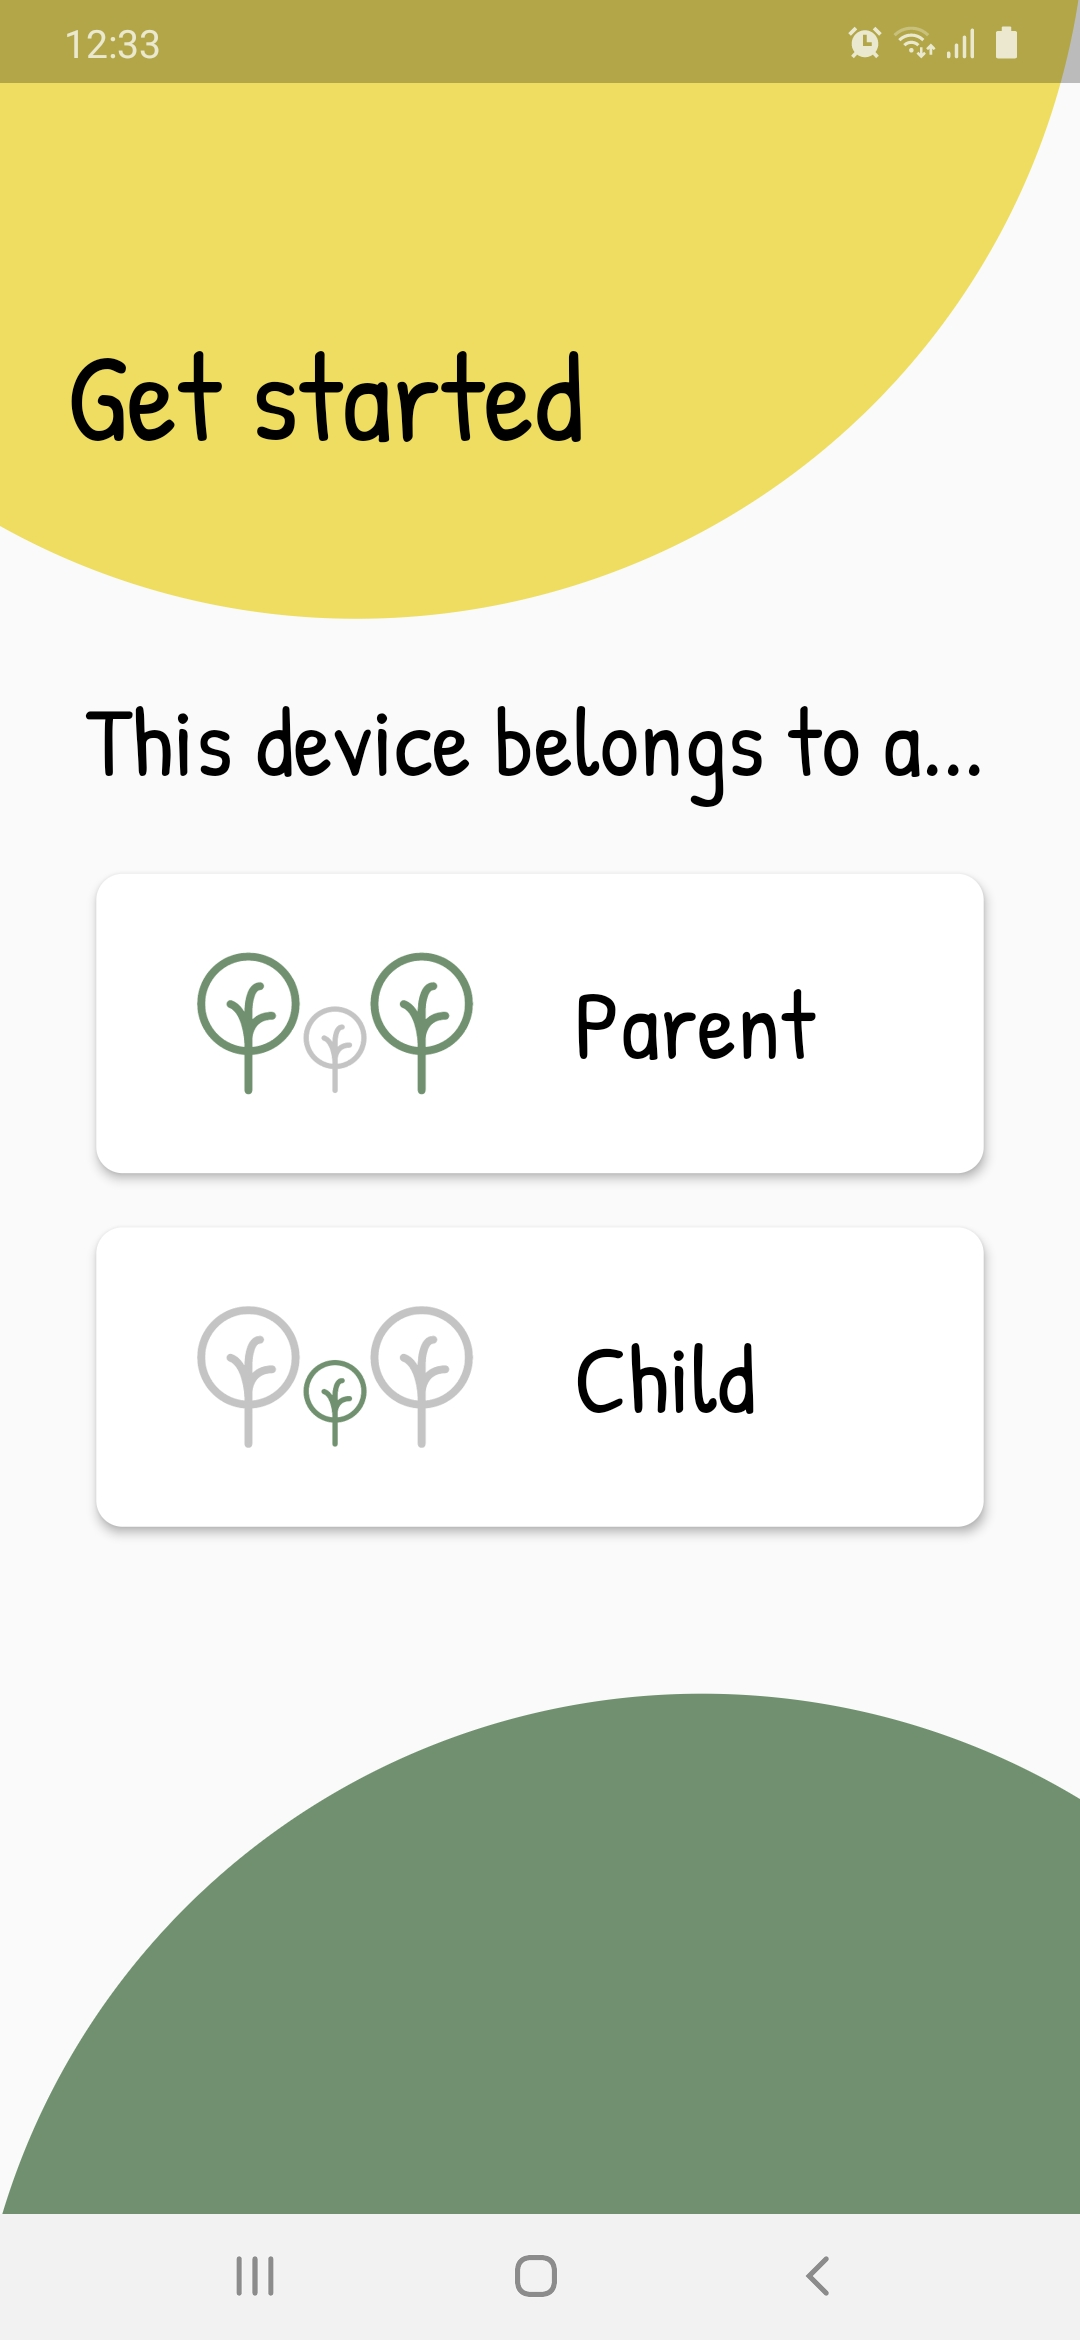
\includegraphics[width=.295\linewidth]{images/cross-device/SGA50/belonging.jpg}} 
&
\subcaptionbox{Login screen\label{fig:cross-device:sga50:login}}{ 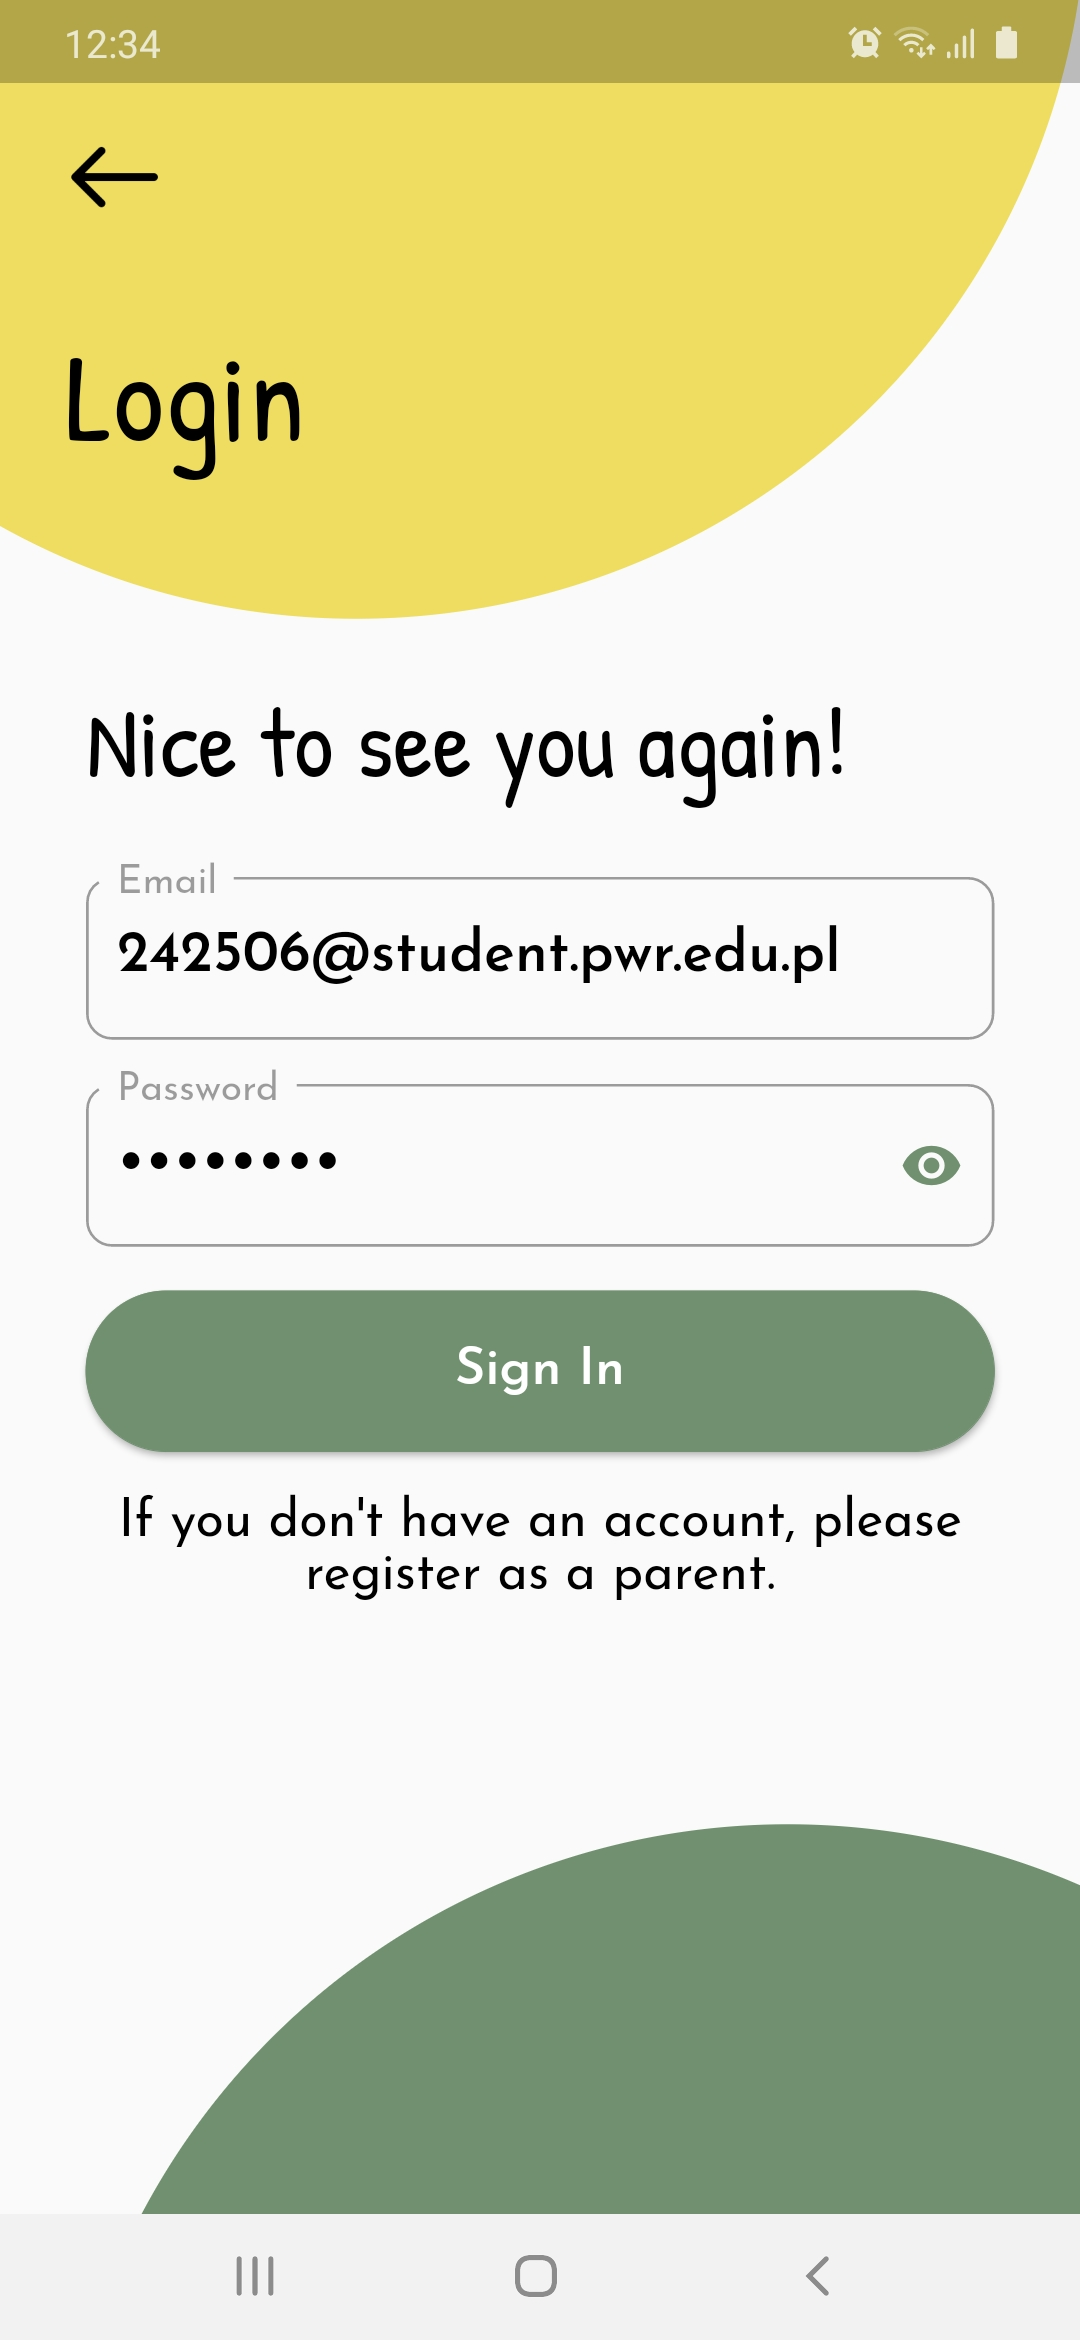
\includegraphics[width=.295\linewidth]{images/cross-device/SGA50/login.jpg}} 
&
\subcaptionbox{Children's profiles list screen\label{fig:cross-device:sga50:profiles}}{ 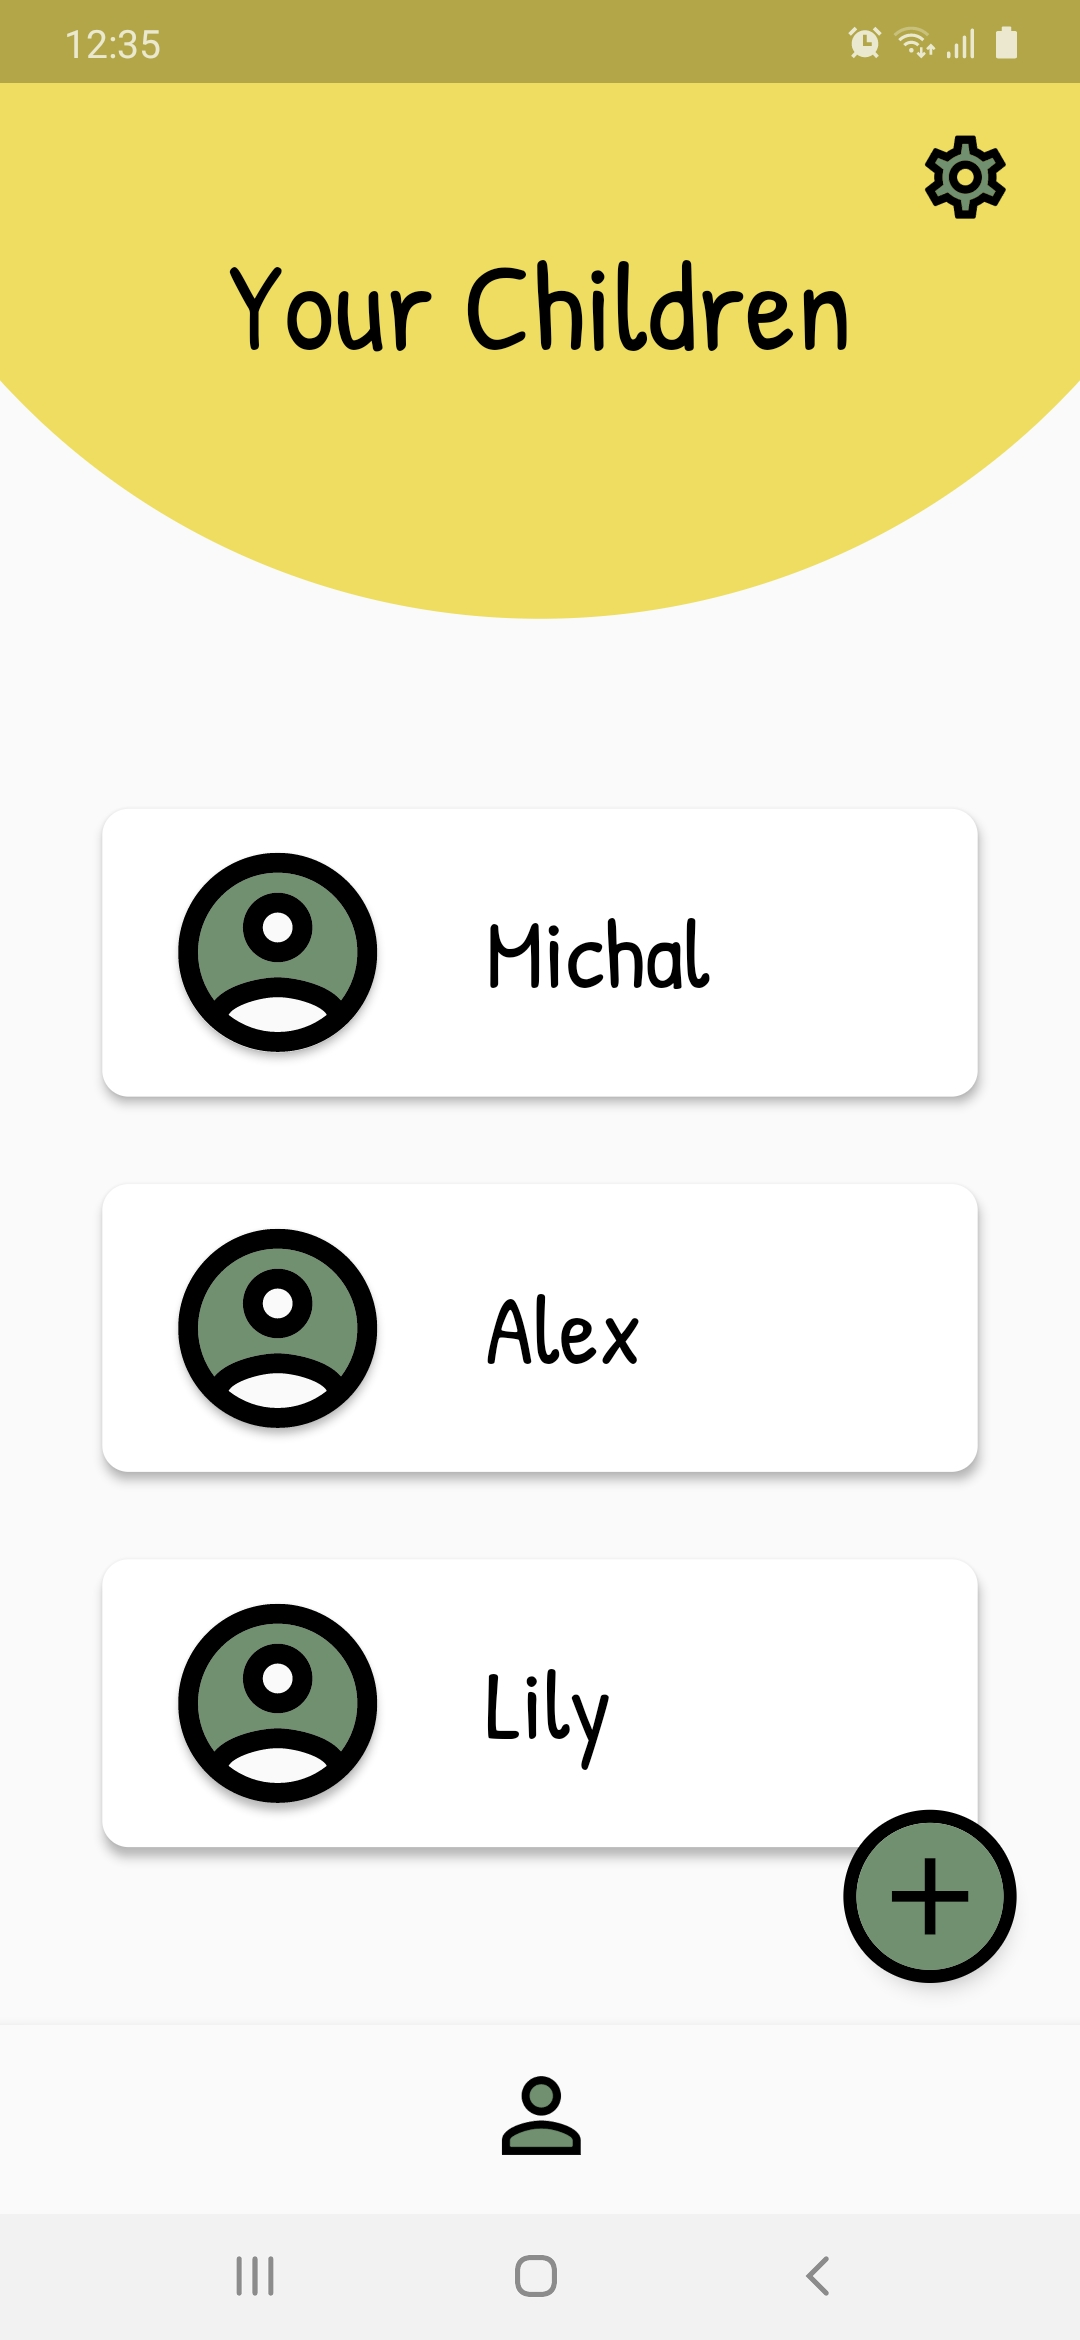
\includegraphics[width=.295\linewidth]{images/cross-device/SGA50/profiles.jpg}} 

\\\\\\\\
\subcaptionbox{Child's tasks screen\label{fig:cross-device:sga50:tasks}}{ 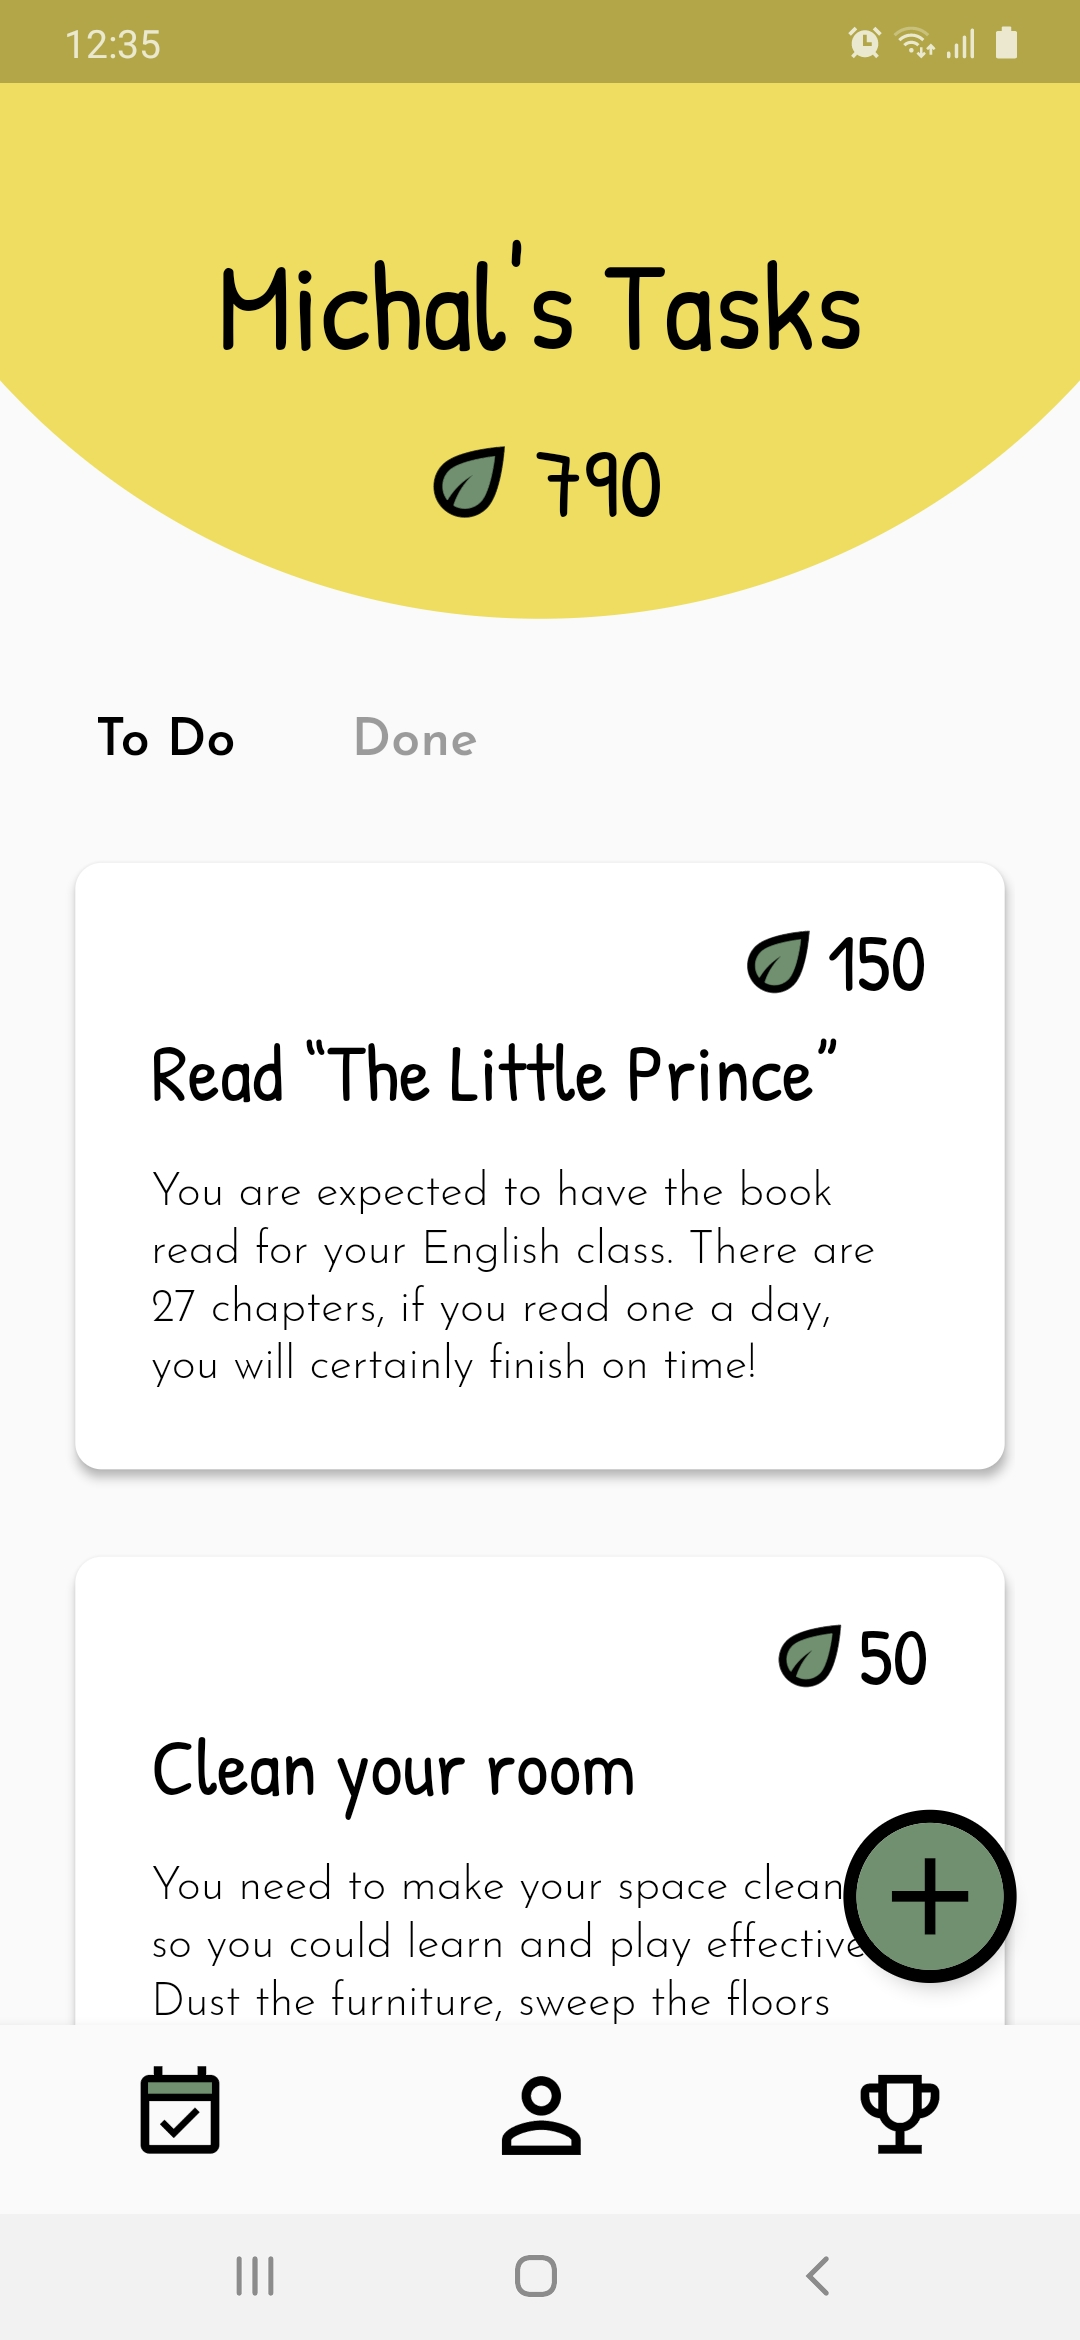
\includegraphics[width=.295\linewidth]{images/cross-device/SGA50/tasks.jpg}} 
&
\subcaptionbox{Task edit screen\label{fig:cross-device:sga50:edit-task}}{ 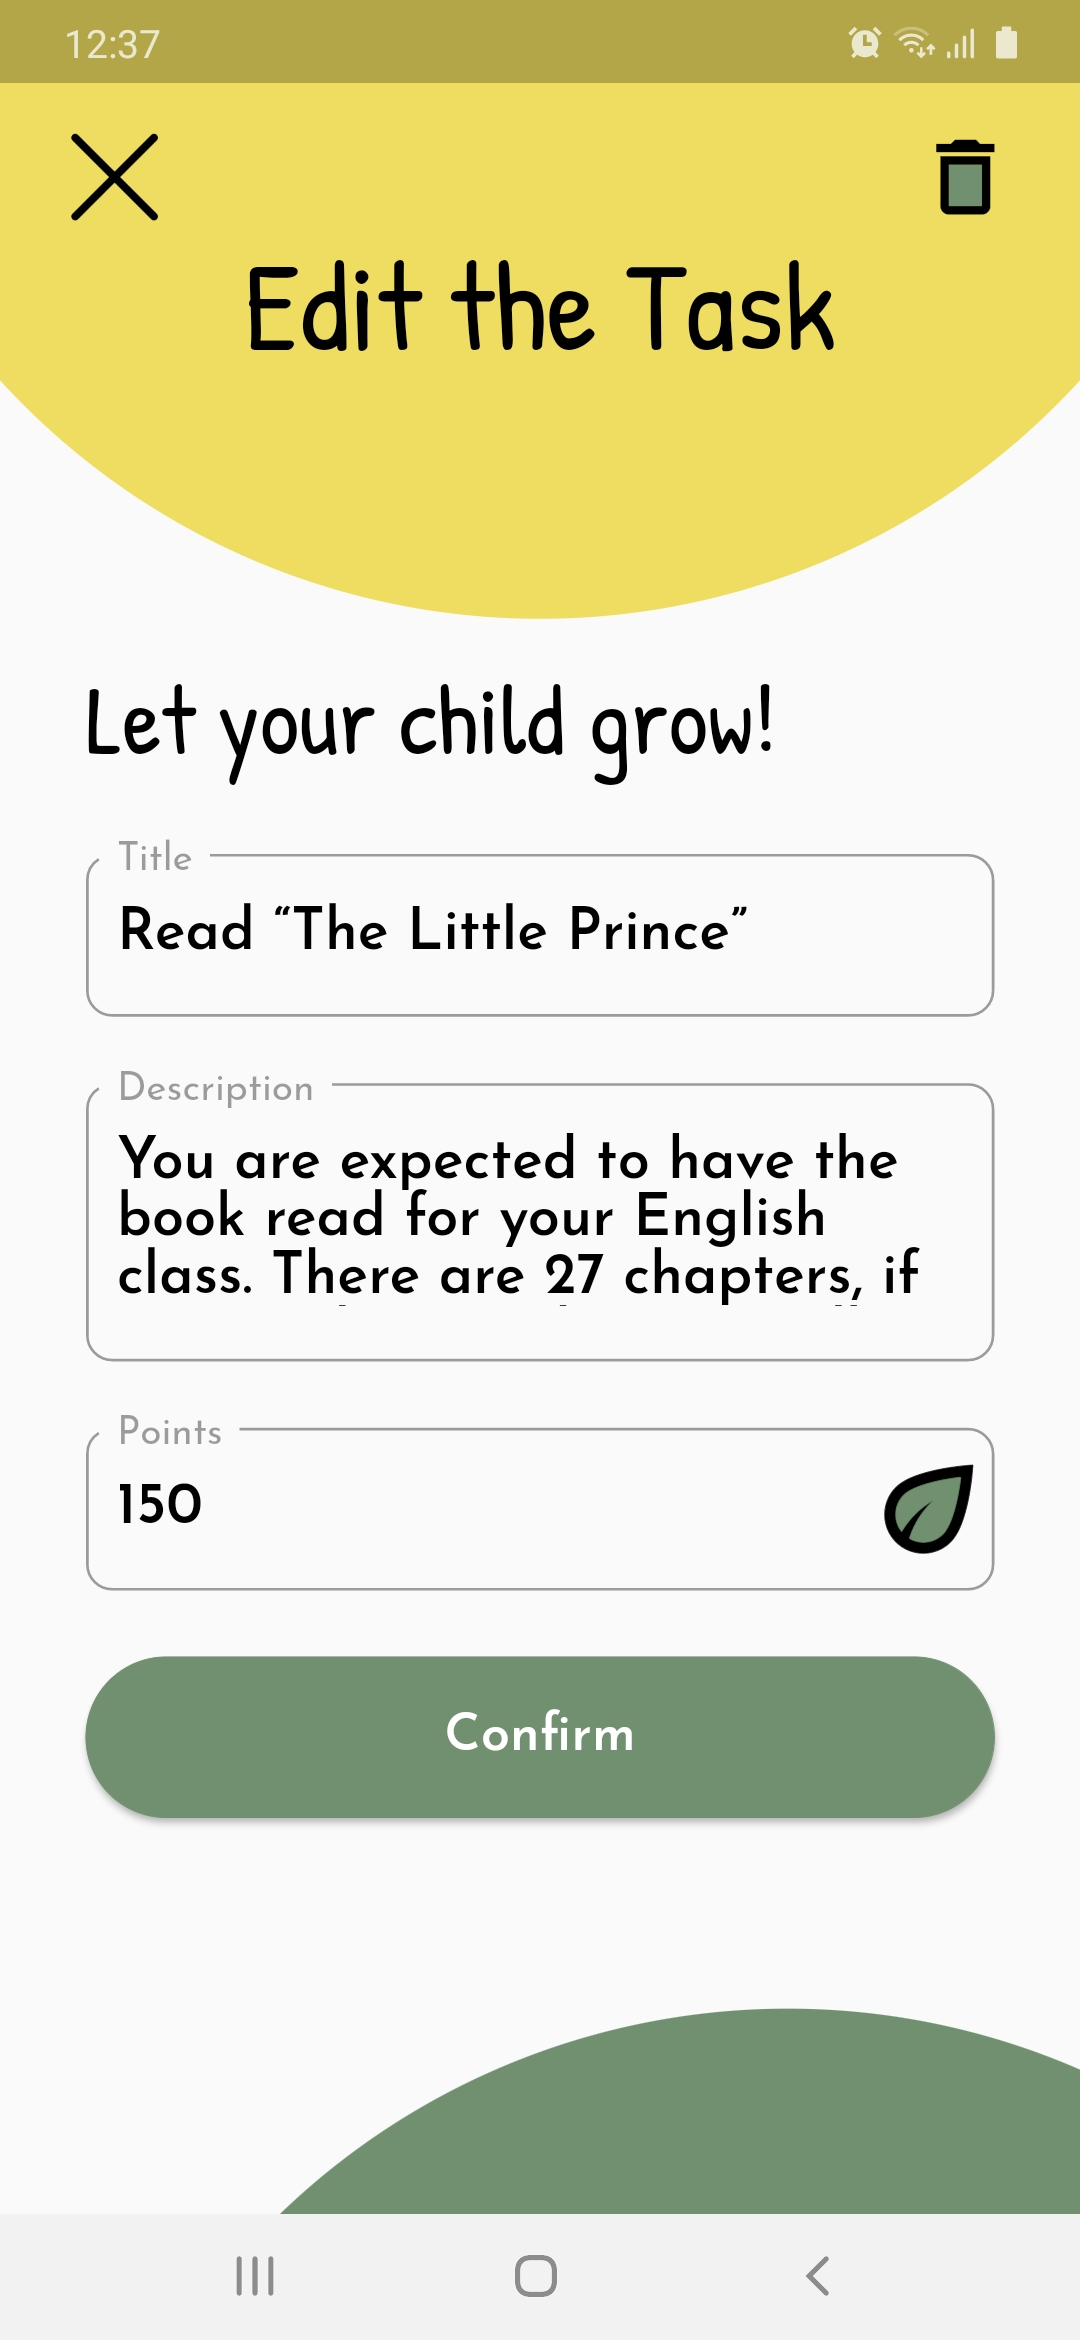
\includegraphics[width=.295\linewidth]{images/cross-device/SGA50/edit_task.jpg}} 
&
\subcaptionbox{Delete task confirmation\label{fig:cross-device:sga50:delete-task}}{ 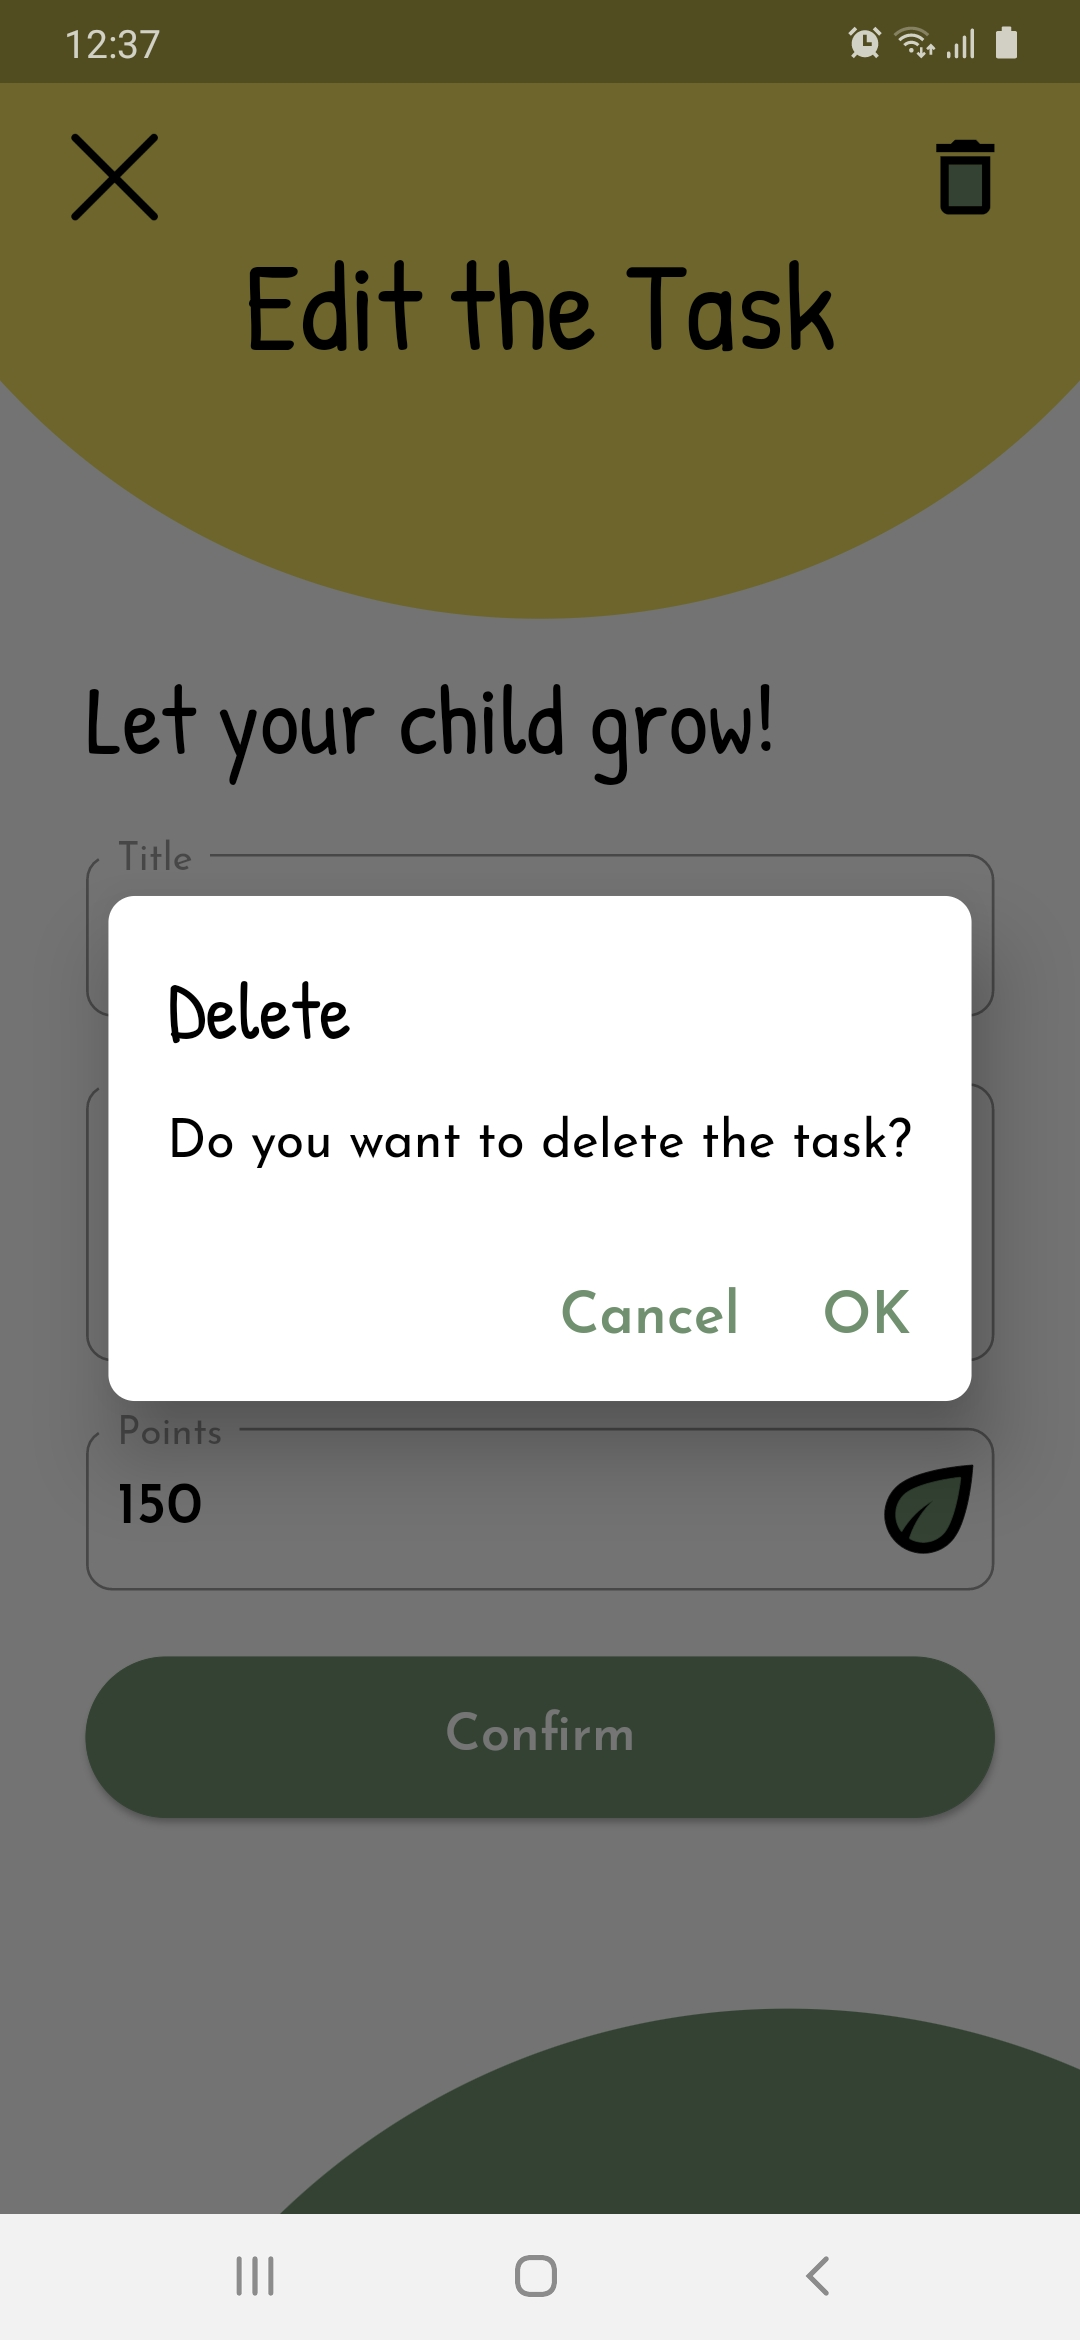
\includegraphics[width=.295\linewidth]{images/cross-device/SGA50/delete_task.jpg}} 
\end{tabular}
\caption{\textit{Raise App} selected screens displayed on Samsung Galaxy A50}
\label{fig:cross-device:sga50}
\end{figure}
\begin{figure}
\captionsetup[subfigure]{justification=centering}
\centering
\begin{tabular}{ccc}
\subcaptionbox{Belonging screen\label{fig:cross-device:sgs5:belonging}}{ 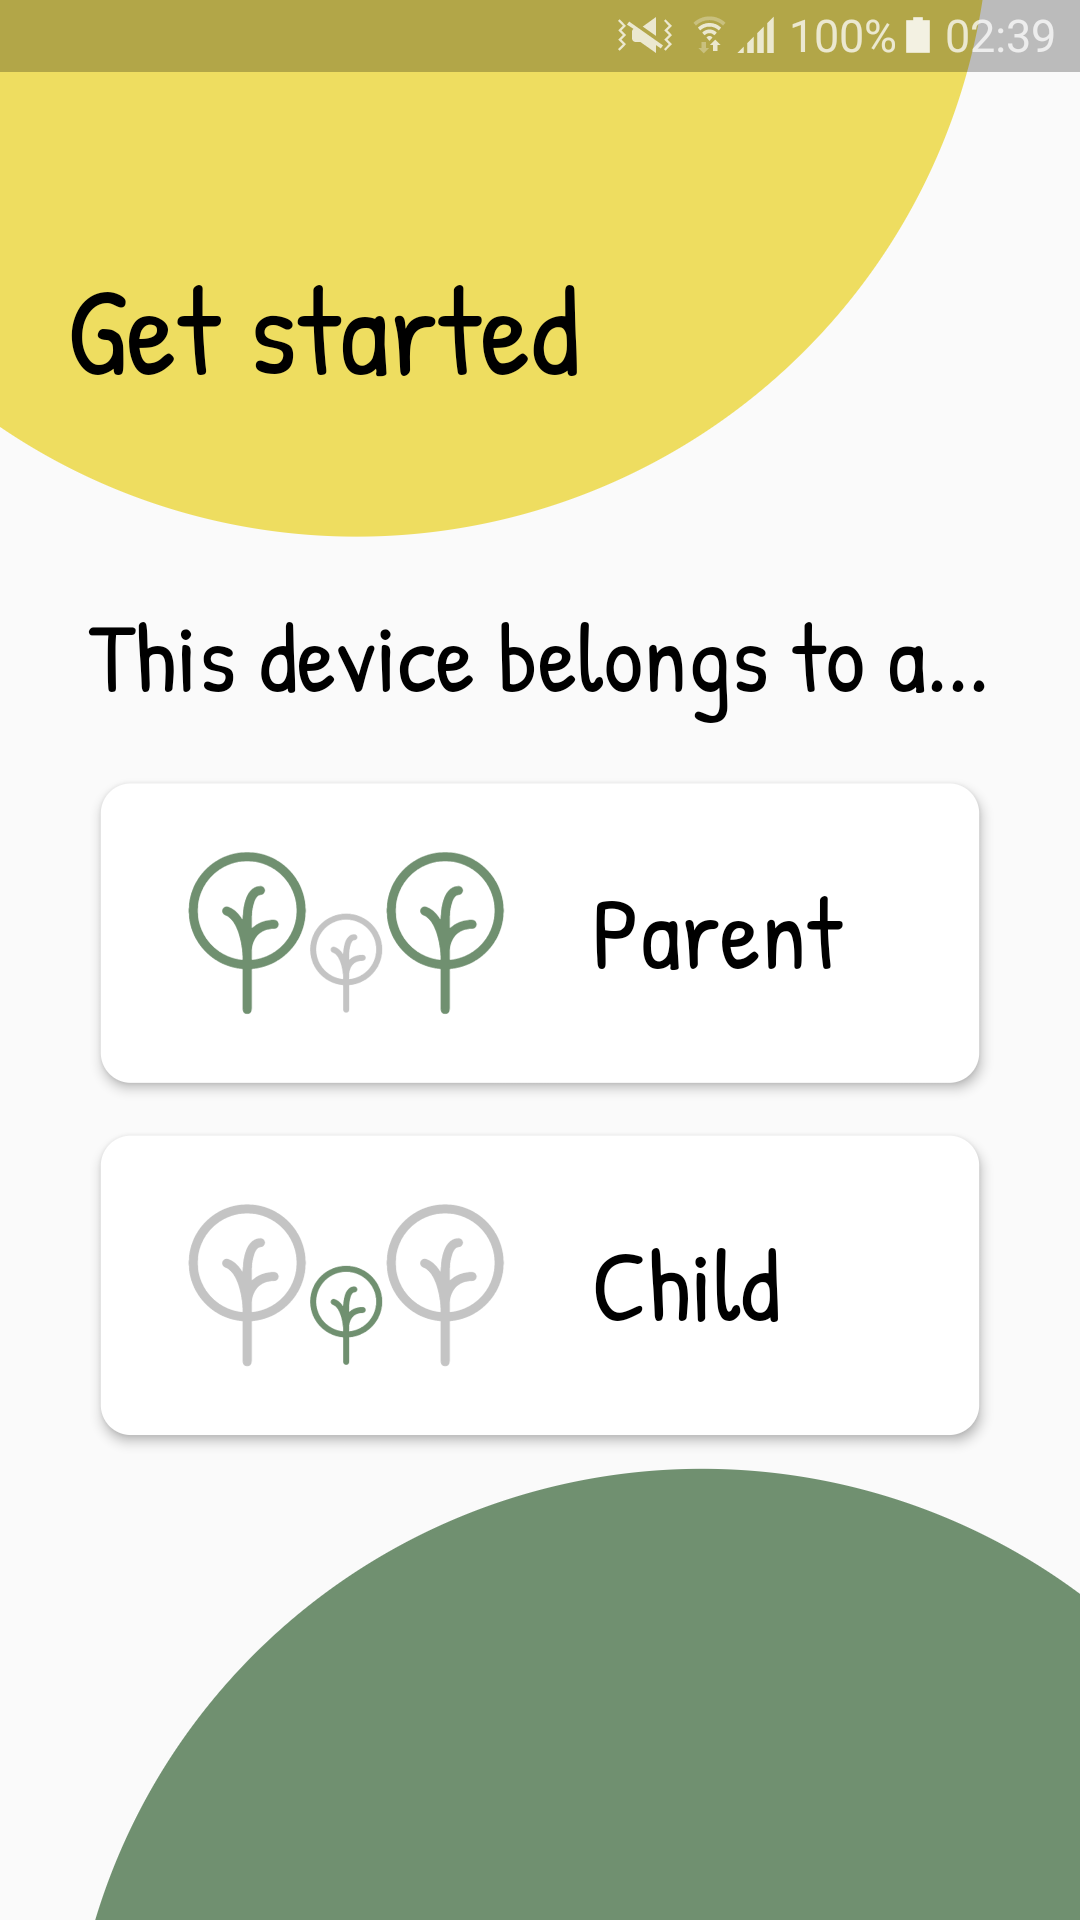
\includegraphics[width=.295\linewidth]{images/cross-device/SGS5/belonging.png}} 
&
\subcaptionbox{Login screen\label{fig:cross-device:sgs5:login}}{ 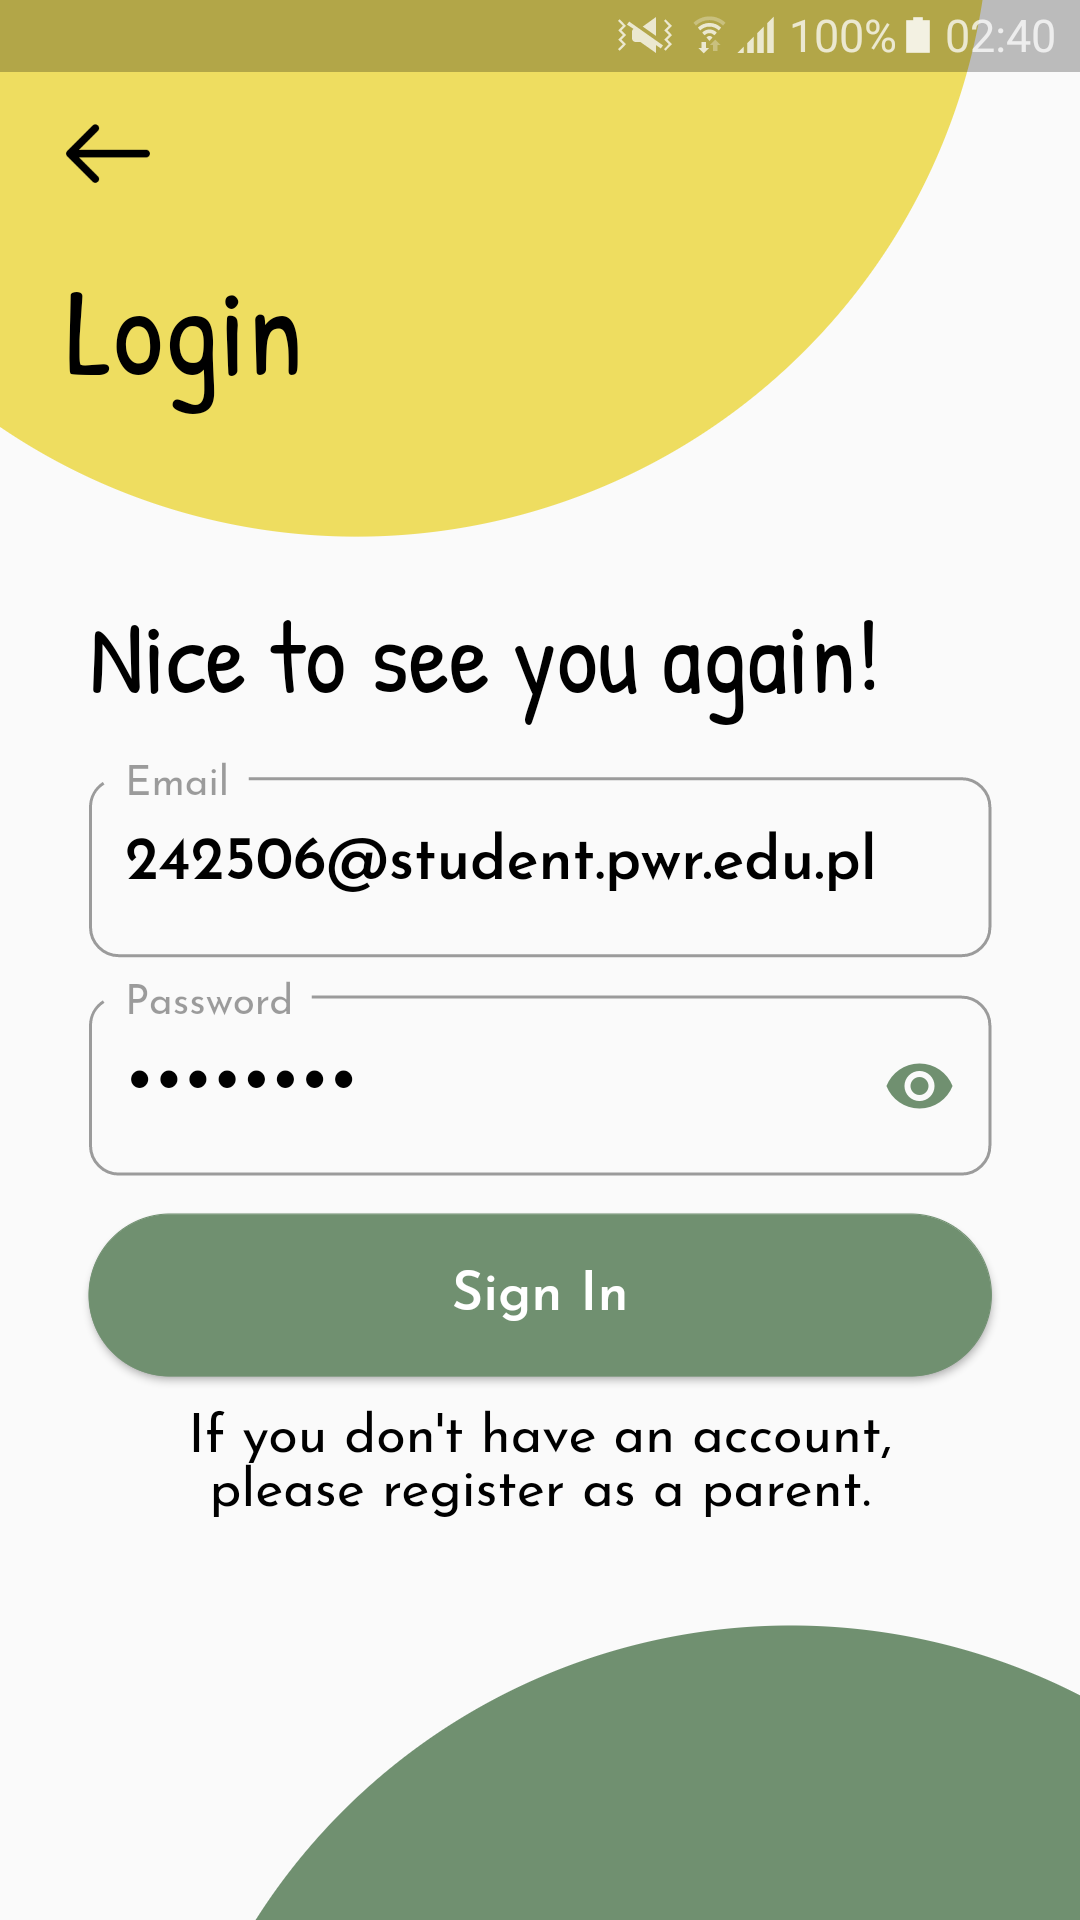
\includegraphics[width=.295\linewidth]{images/cross-device/SGS5/login.png}} 
&
\subcaptionbox{Children's profiles list screen\label{fig:cross-device:sgs5:profiles}}{ 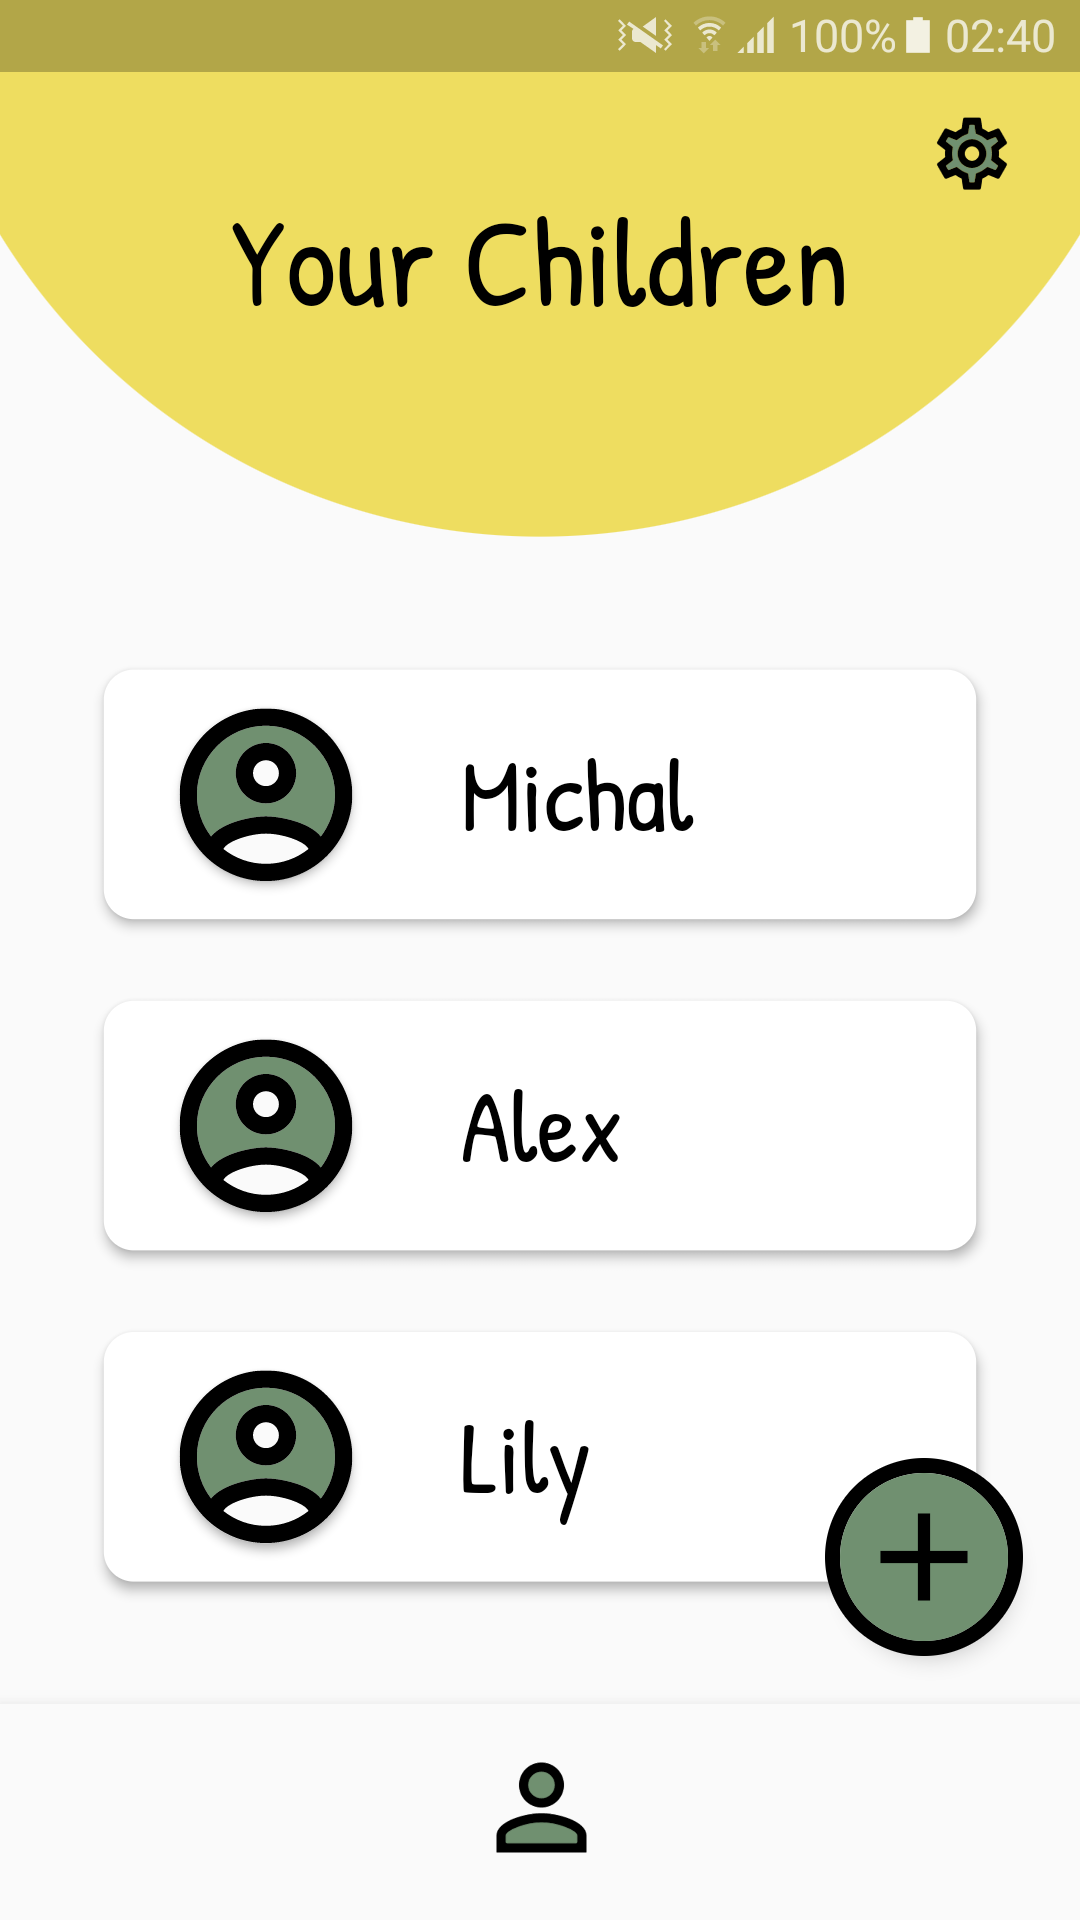
\includegraphics[width=.295\linewidth]{images/cross-device/SGS5/profiles.png}} 

\\\\\\\\
\subcaptionbox{Child's tasks screen\label{fig:cross-device:sgs6:tasks}}{ 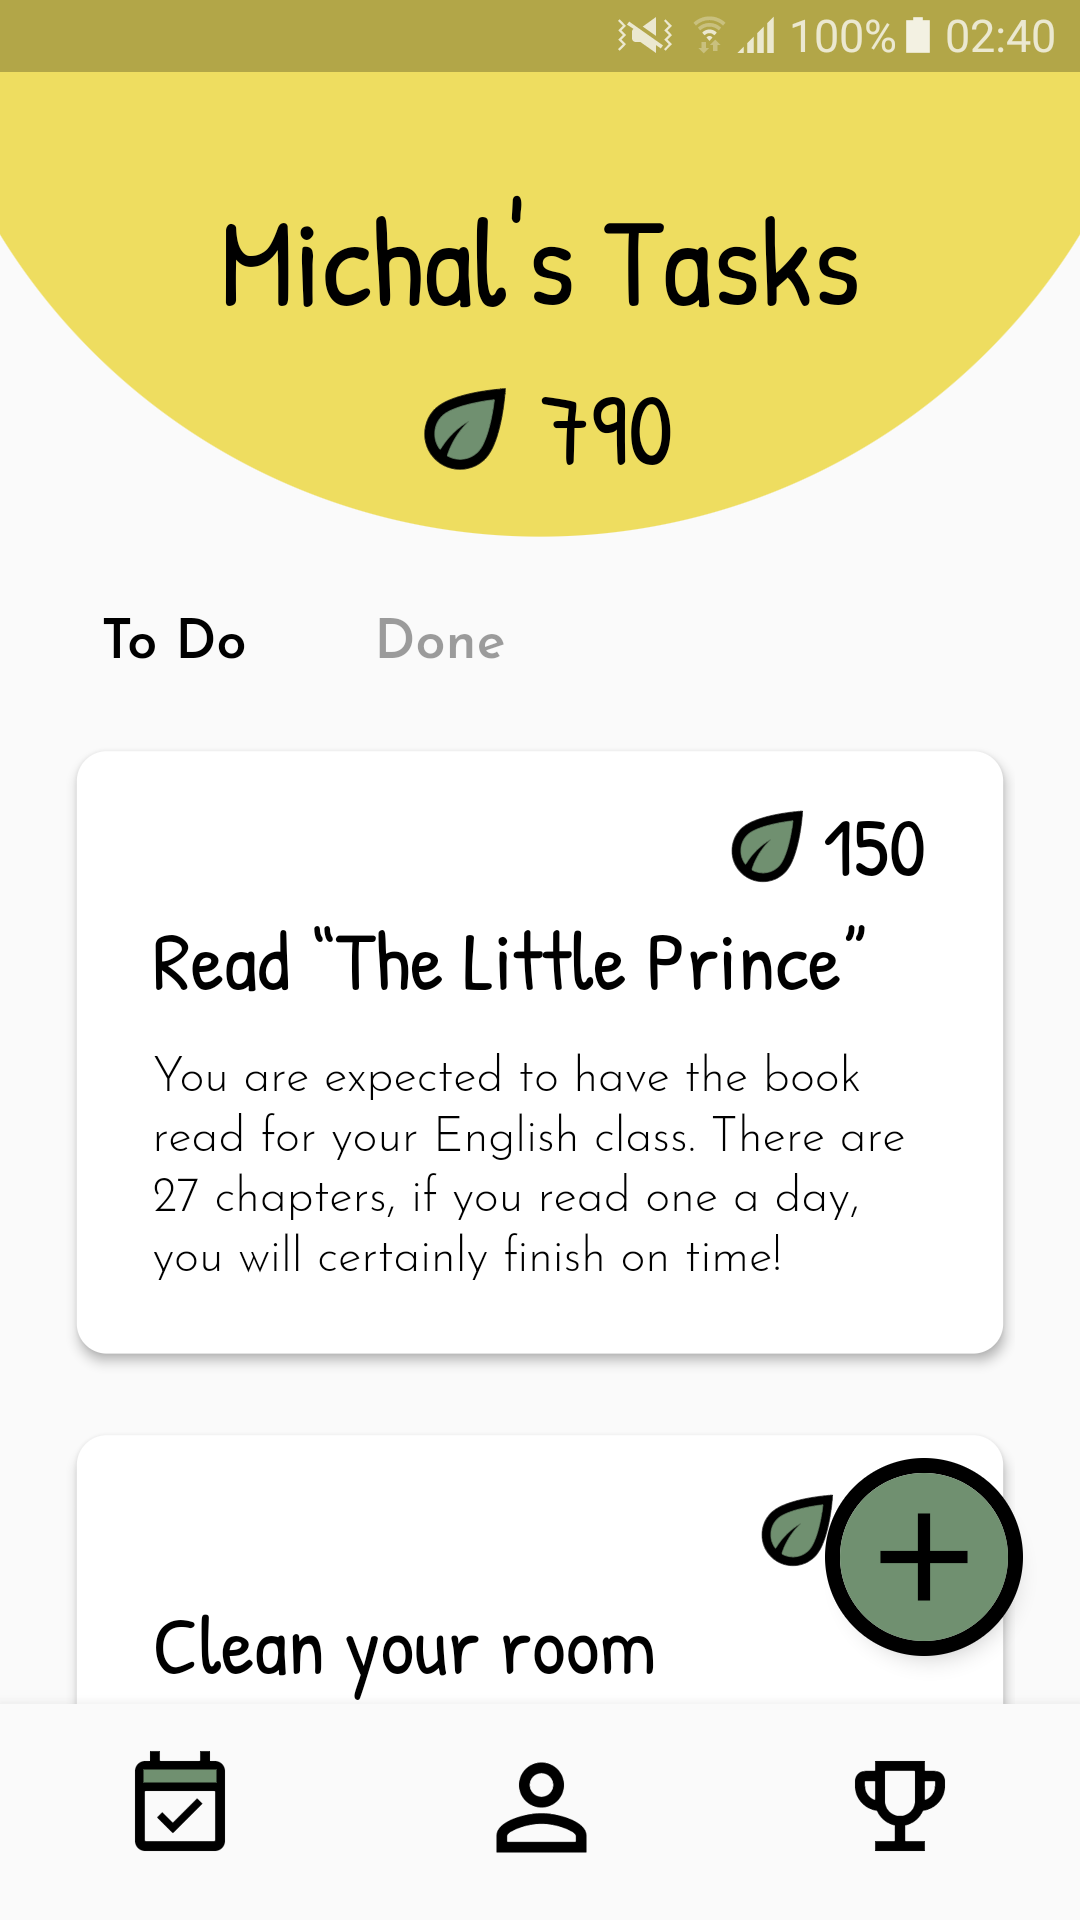
\includegraphics[width=.295\linewidth]{images/cross-device/SGS5/tasks.png}} 
&
\subcaptionbox{Task edit screen\label{fig:cross-device:sgs5:edit-task}}{ 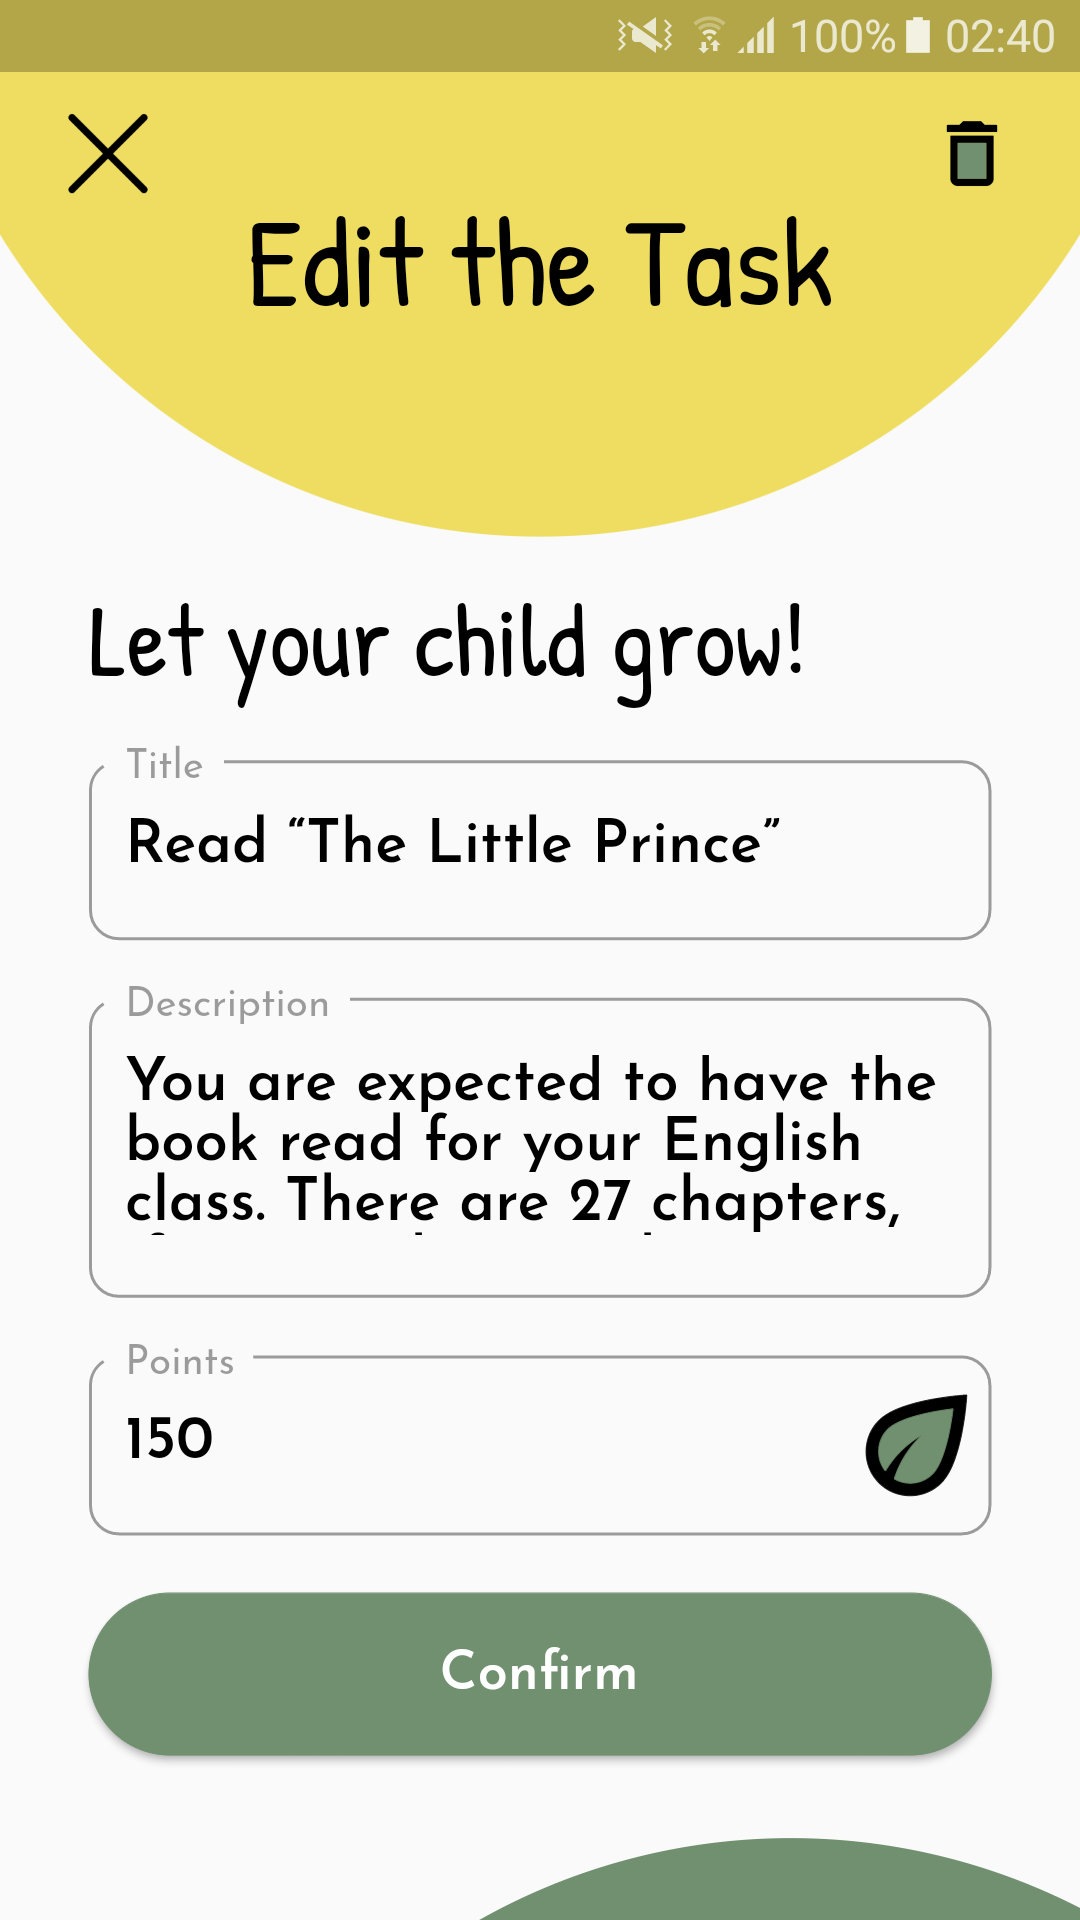
\includegraphics[width=.295\linewidth]{images/cross-device/SGS5/edit_task.png}} 
&
\subcaptionbox{Delete task confirmation\label{fig:cross-device:sgs5:delete-task}}{ 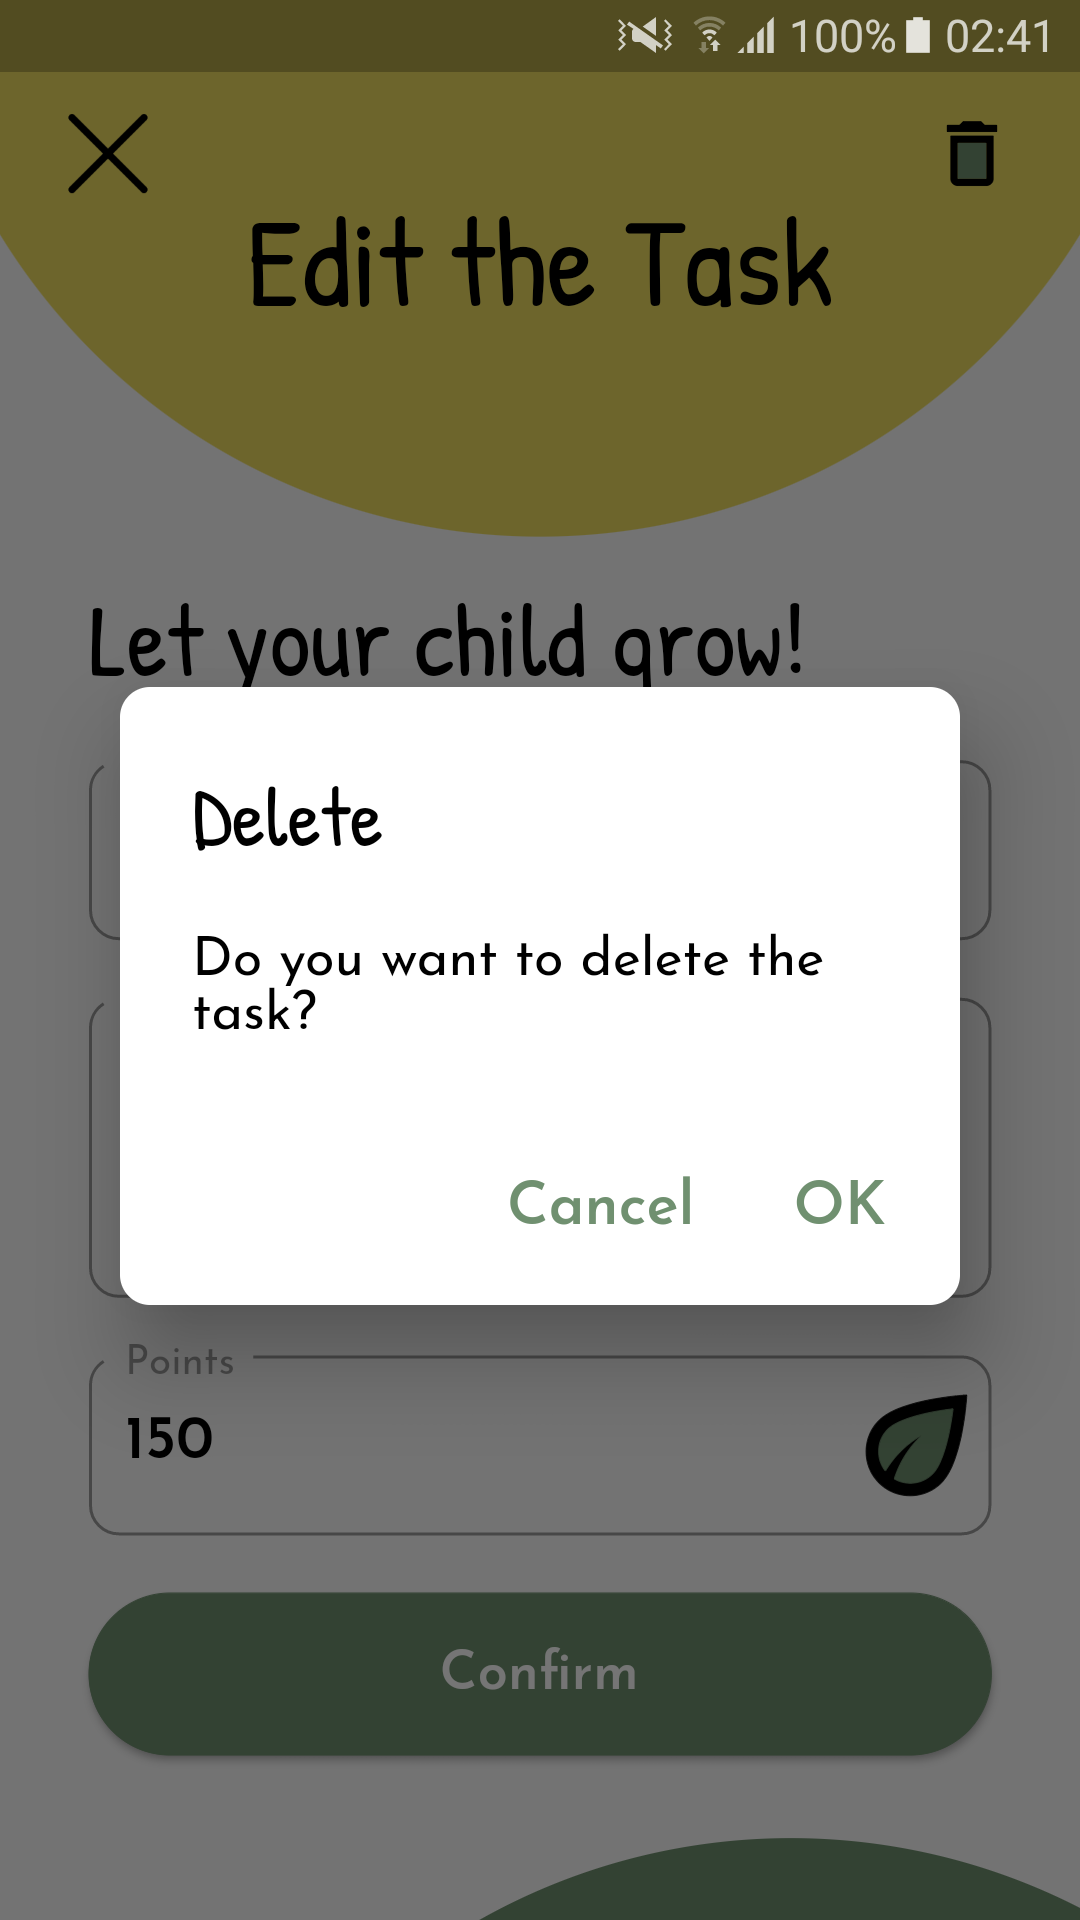
\includegraphics[width=.295\linewidth]{images/cross-device/SGS5/delete_task.png}} 
\end{tabular}
\caption{\textit{Raise App} selected screens displayed on Samsung Galaxy S5}
\label{fig:cross-device:sgs5}
\end{figure}
\begin{figure}
\captionsetup[subfigure]{justification=centering}
\centering
\begin{tabular}{ccc}
\subcaptionbox{Belonging screen\label{fig:cross-device:fwvga37:belonging}}{ 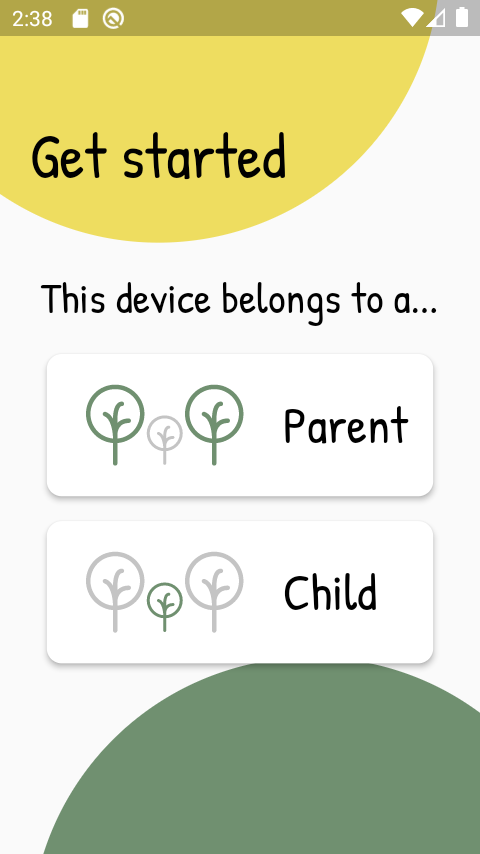
\includegraphics[width=.295\linewidth]{images/cross-device/FWVGA37/belonging.png}} 
&
\subcaptionbox{Login screen\label{fig:cross-device:fwvga37:login}}{ 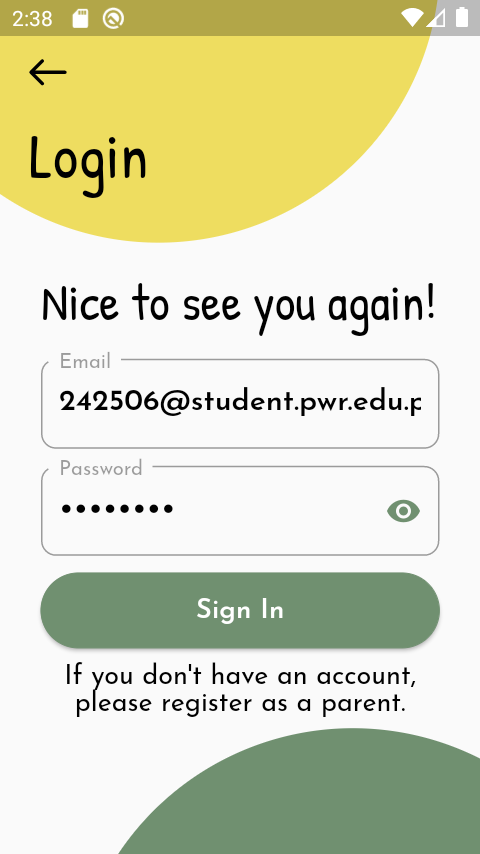
\includegraphics[width=.295\linewidth]{images/cross-device/FWVGA37/login.png}} 
&
\subcaptionbox{Children's profiles list screen\label{fig:cross-device:fwvga37:profiles}}{ 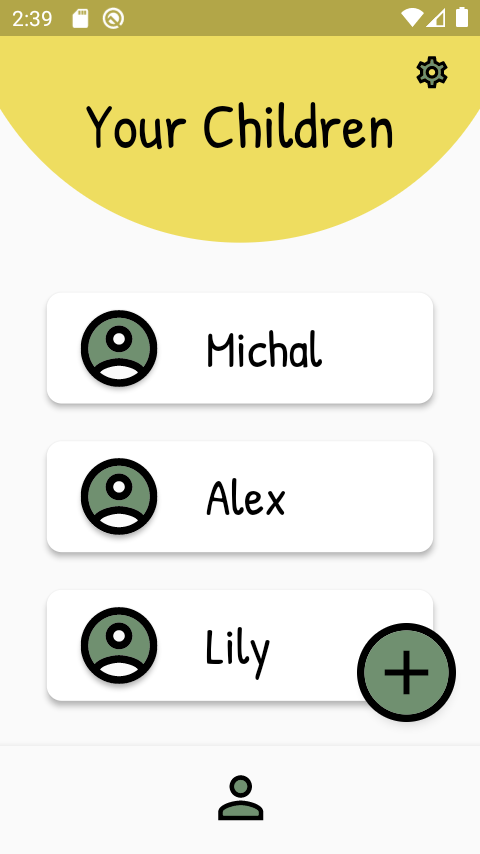
\includegraphics[width=.295\linewidth]{images/cross-device/FWVGA37/profiles.png}} 

\\\\\\\\
\subcaptionbox{Child's tasks screen\label{fig:cross-device:sgs6:tasks}}{ 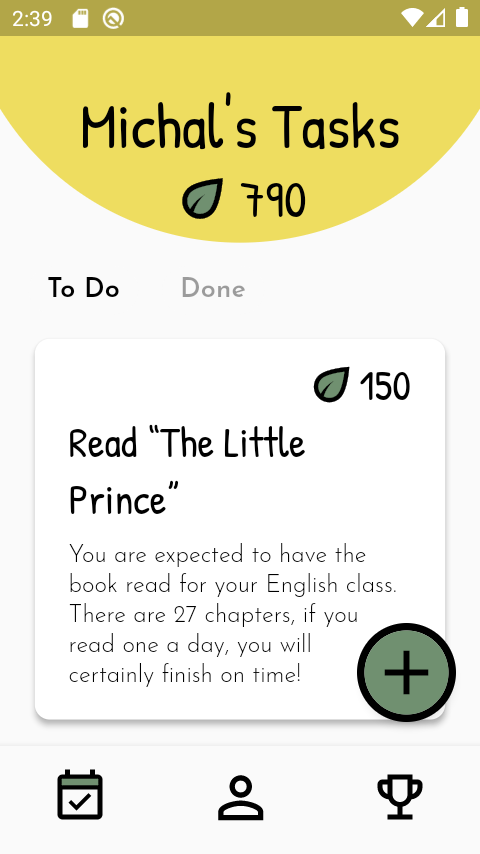
\includegraphics[width=.295\linewidth]{images/cross-device/FWVGA37/tasks.png}} 
&
\subcaptionbox{Task edit screen\label{fig:cross-device:fwvga37:edit-task}}{ 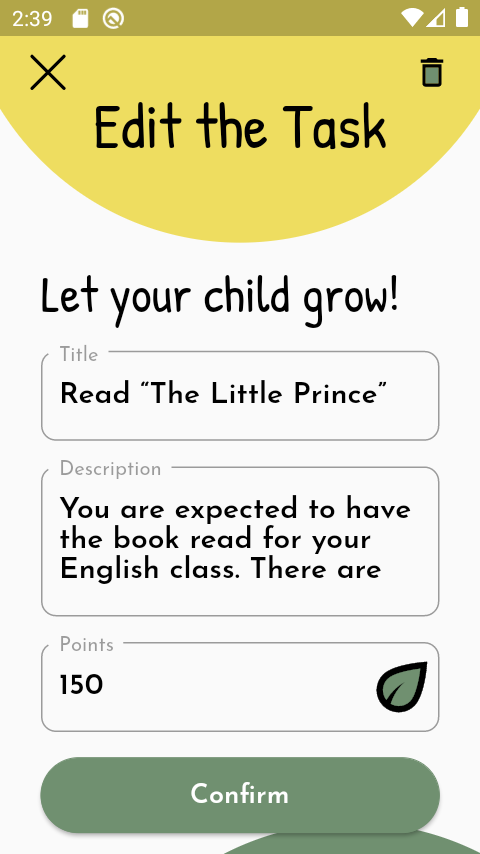
\includegraphics[width=.295\linewidth]{images/cross-device/FWVGA37/edit_task.png}} 
&
\subcaptionbox{Delete task confirmation\label{fig:cross-device:fwvga37:delete-task}}{ 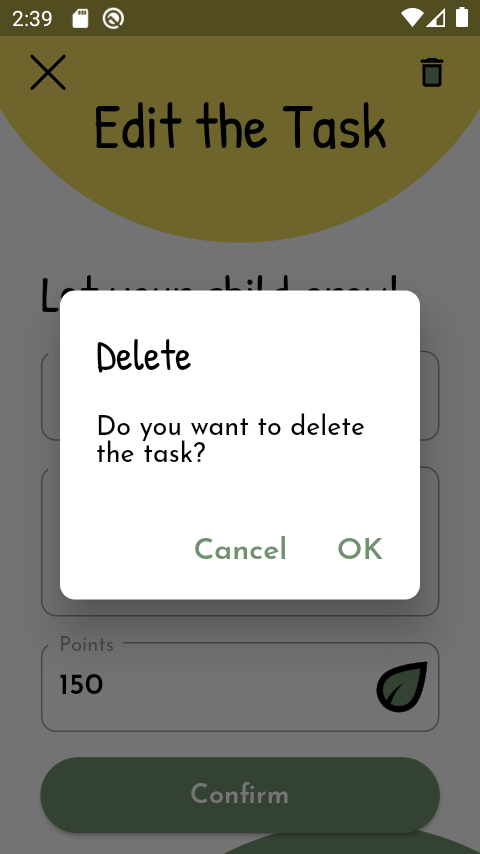
\includegraphics[width=.295\linewidth]{images/cross-device/FWVGA37/delete_task.png}} 
\end{tabular}
\caption{\textit{Raise App} selected screens displayed on the emulated device}
\label{fig:cross-device:fwvga37}
\end{figure}


\section{User Acceptance tests}\label{sec:tests:user}
\textit{User acceptance tests} is a process of verifying that a solution works for the end user. One of the most important metrics of this is \textit{usability} and \textit{user experience}. The former is a term precisely defined in the \textit{ISO 9126}, \say{Software engineering — Product quality} and \textit{ISO 9241}, \say{Ergonomics of Human System Interaction} standards \cite{idriUseSoftwareQuality2013,moumaneUsabilityEvaluationMobile2016}. They distinguish four aspects of usability:
\begin{itemize}
    \item Understandability
    \item Learnability
    \item Operability
    \item Attractiveness
\end{itemize}
The standards, however, do not provide implementations of usability test.
\\\\
\say{Userbility: A Technique for the Evaluation of User Experience and Usability on Mobile Applications} is the name of a 2016 article that, based on the aforementioned standards, introduces a new approach to usability and user experience testing. It proposes using \say{selected questions aim to assist in capturing the experience and emotions of
non-specialist evaluators about the application} \cite{nascimentoUserbilityTechniqueEvaluation2016}.
\\\\
Inspired by those, a questionnaire aiming to test both the usability and user experience of the created application was built and sent out to the first users of the application. The following sections will describe its structure and summarize the results.

\subsection{Questionnaire structure}
The questionnaire was prepared on the Google Forms platform and, at the time of the writing, can be found under \href{https://forms.gle/vUELFR6BDmpUxsam6}{this link}\footnote{https://forms.gle/vUELFR6BDmpUxsam6 (accessed Dec. 13, 2020)}  (also, as the audience was partly Polish, a translated version can be found \href{https://forms.gle/gGbony1Ktq47MmwBA}{here}\footnote{https://forms.gle/gGbony1Ktq47MmwBA (accessed Dec. 13, 2020)}).
\\\\
The form consists of:
\begin{enumerate}
    \item An introduction explaining the questionnaire's goal and structure.
    \item Five sections, whose structure is based on the \textit{userbility} technique, regarding:
    \begin{itemize}
        \item attractiveness
        \item understandability
        \item learnability
        \item in-app communication
        \item performance
    \end{itemize}
    \item An overall mark.
    \item A \textit{support} section, where users can provide feedback regardless of the asked questions.
\end{enumerate}
\\\\
The most important, from the evaluation point of view, are the five sections measuring usability. Each of starts with a brief explanation of the term it is concerning, followed by three questions that have a following structure:
\begin{enumerate}
    \item What do you feel regarding the \textit{measure} of the application?
    \item What do you think could improve the \textit{measure} of the application?
    \item How satisfied are you with the \textit{measure} of the application?
\end{enumerate}
where \textit{measure} is one of the five aforementioned usability measures. First two, not mandatory, questions are open-ended and allow for expressing the user's opinion, while the last, mandatory, question is a mark, ranging from 1 (\say{extremely unsatisfied}) to 10 (\say{extremely satisfied}).


\subsection{Results}
At the time of writing\footnote{Dec. 13, 2020}, 21 answers have been gathered. The results will be broken down into section, according to the questionnaire's structure.


\subsubsection{Attractiveness}
The arithmetic average of the users' marks for the attractiveness was \textbf{8.86}. The users highlighted the interface, its simplicity, elegance and modernity. They praised the colour and font choices. Many were attracted by the design. Some of them noted that the loading animation should be more pronounced. One user asked for a colour customisation option depending on a child.


\subsubsection{Understandability}
The arithmetic average of the users' marks for the attractiveness was \textbf{8.0}. Users were able to understand how the application can be used for the particular tasks and conditions of use. However, there were reports of a need for an onboarding process of some sort. Users expected an explanation of certain elements of the application (i.e. reward filters) and how could they benefit from them.


\subsubsection{Learnability}
The arithmetic average of the users' marks for the learnability was \textbf{8.1}. Users were generally satisfied with the learnability process. They could quickly get familiar with the application and make good use of most of its features. Because nearly half of the testers were Polish, one of the most frequent remarks was about introducing translations to the applications. One user mentioned being confused about the \textit{add} button, which allowed for adding elements not related to the displayed screen (i.e. rewards on the tasks screen).


\subsubsection{In-app Communication}
The arithmetic average of the users' marks for the in-app communication was \textbf{8.71}. In general, users were very satisfied with the amount of information about what has happened or is going to happen. They praised the clarity of messages. One user highlighted the confirmation alert appearing before the app is closed, as it prevents accidental exits. Some users expressed a need for \say{help} tooltips. 


\subsubsection{Performance}
The arithmetic average of the users' marks for the application performance was \textbf{8.8}. Users did not notice any performance issues, and if, they were usually related to their internet connection. They did not notice any delays during the application execution, or an increased battery usage. 


\subsubsection{Overall}
The arithmetic average of the users' marks for overall satisfaction was \textbf{9.14}. This is the highest average of all the categories and suggest that despite sparse shortcomings, they have positive associations with the applications, which is important on the current market, where most of the decisions are made on a sub-conscious level. 


\section{Summary}\label{sec:tests:summary}
Tests introduced to the project provided a much higher quality of the final product. It was important to introduce them on different levels, in order to maintain a broad perspective of the feedback loop. Unit and widget tests ensured correctness of execution of the functions, methods and widgets on the lowest level of granularity. Integration tests allowed for a more comprehensive check of the system elements' interoperability. Cross-device tests confirmed that the application will work on the expected devices, specified in the requirements. Finally, the user acceptance tests provided the target group feedback, which will set direction to the future development of the product.